\section{Saving measures}
\subsection{Introduction}
With our existing approaches we are able to translate any Kandinsky drawing with arbitrary degree to a smooth orthogonal layout with a complexity increase by 2 for larger polyedges in $\Rho(n^2)\times\Rho(n)$ area. The question arises whether it was possible to even save some bends or find a method to stretch with less area requirements in the worst case. In the following section, we examine possibilities to decrease the complexity of polyedges. Furthermore we try to lower the area upper bound in a possible tradeoff with some more bends.
\subsection{Edge Complexity Bounds}
Reconsider the drawing given in Figure \ref{im:kandinsky_bends2}. Due to the fact that the previous results considering 4-planar graphs are also holding for graphs of arbitrary degree, the results are applicable.\\
\begin{figure}[H]
	\centering
	\begin{subfigure}{0.6\linewidth}
		\centering
		\includegraphics[width=0.7\textwidth,page=2]{includegraphics/kandinsky_bends_arbitrary.pdf}
	\end{subfigure}
	\caption{Recall Figure \ref{im:kandinsky_bends2}}\label{im:recall1}
\end{figure}
\begin{theorem}
	Every Kandinsky drawing of a complexity-3 graph with arbitrary degree can be postprocessed to a complexity-4 smooth orthogonal layout in $\Rho(n^2)\times\Rho(n)$ area.
\end{theorem}
\begin{proof}
	Just as the proof of Theorem \ref{th:3to4} holds, the Kandinsky bends are not erasable, leading to a staircase situation of complexity 3. The boxing brings along one more bend, resulting in a polyedge of complexity 4.
\end{proof}
The difference in our new situation is that we are able to reposition the polyedges on the ports. By having a 4-planar graph interpreted in Kandinsky, we are able to connect up to four edges on a single port. This gives us a new opportunity to optimize the drawings.
\begin{remark}
	The \textit{bend or end} property complicates the port reassignment possibilities.
\end{remark}
If we recall Figure \ref{im:kandinsky_bends2}, we could try to alter the port the edge is connected to. Unfortunately, the uniformity of the vertex boxes lead to a possible collision illustrated in Figure \ref{im:bend_or_end_collision}. By doing so, we would further increase the complexity of the edge.
\begin{figure}[H]
	\centering
	\begin{subfigure}{0.3\linewidth}
		\centering
		\includegraphics[width=0.4\textwidth,page=3]{includegraphics/kandinsky_bends_arbitrary.pdf}
		\caption{\textit{bend or end} collision}\label{im:bend_or_end_collision}
	\end{subfigure}
	\begin{subfigure}{0.3\linewidth}
		\centering
		\includegraphics[width=0.4\textwidth,page=4]{includegraphics/kandinsky_bends_arbitrary.pdf}
		\caption{Complexity increase}\label{im:bend_or_end_comp_increase}
	\end{subfigure}
	\caption{Bend or end property complicates matters}\label{im:bend_or_end}
\end{figure}
But on the other hand, the circular arcs are flexible enough to achieve a possible complexity decrease.
\begin{figure}[H]
	\centering
	\begin{subfigure}{0.6\linewidth}
		\centering
		\includegraphics[width=0.7\textwidth,page=5]{includegraphics/kandinsky_bends_arbitrary.pdf}
	\end{subfigure}
	\caption{SMOG complexity decreases}
\end{figure}
However, this is not always possible, as we see in the following Figure:
\begin{figure}[H]
	\centering
	\begin{subfigure}{0.45\linewidth}
		\centering
		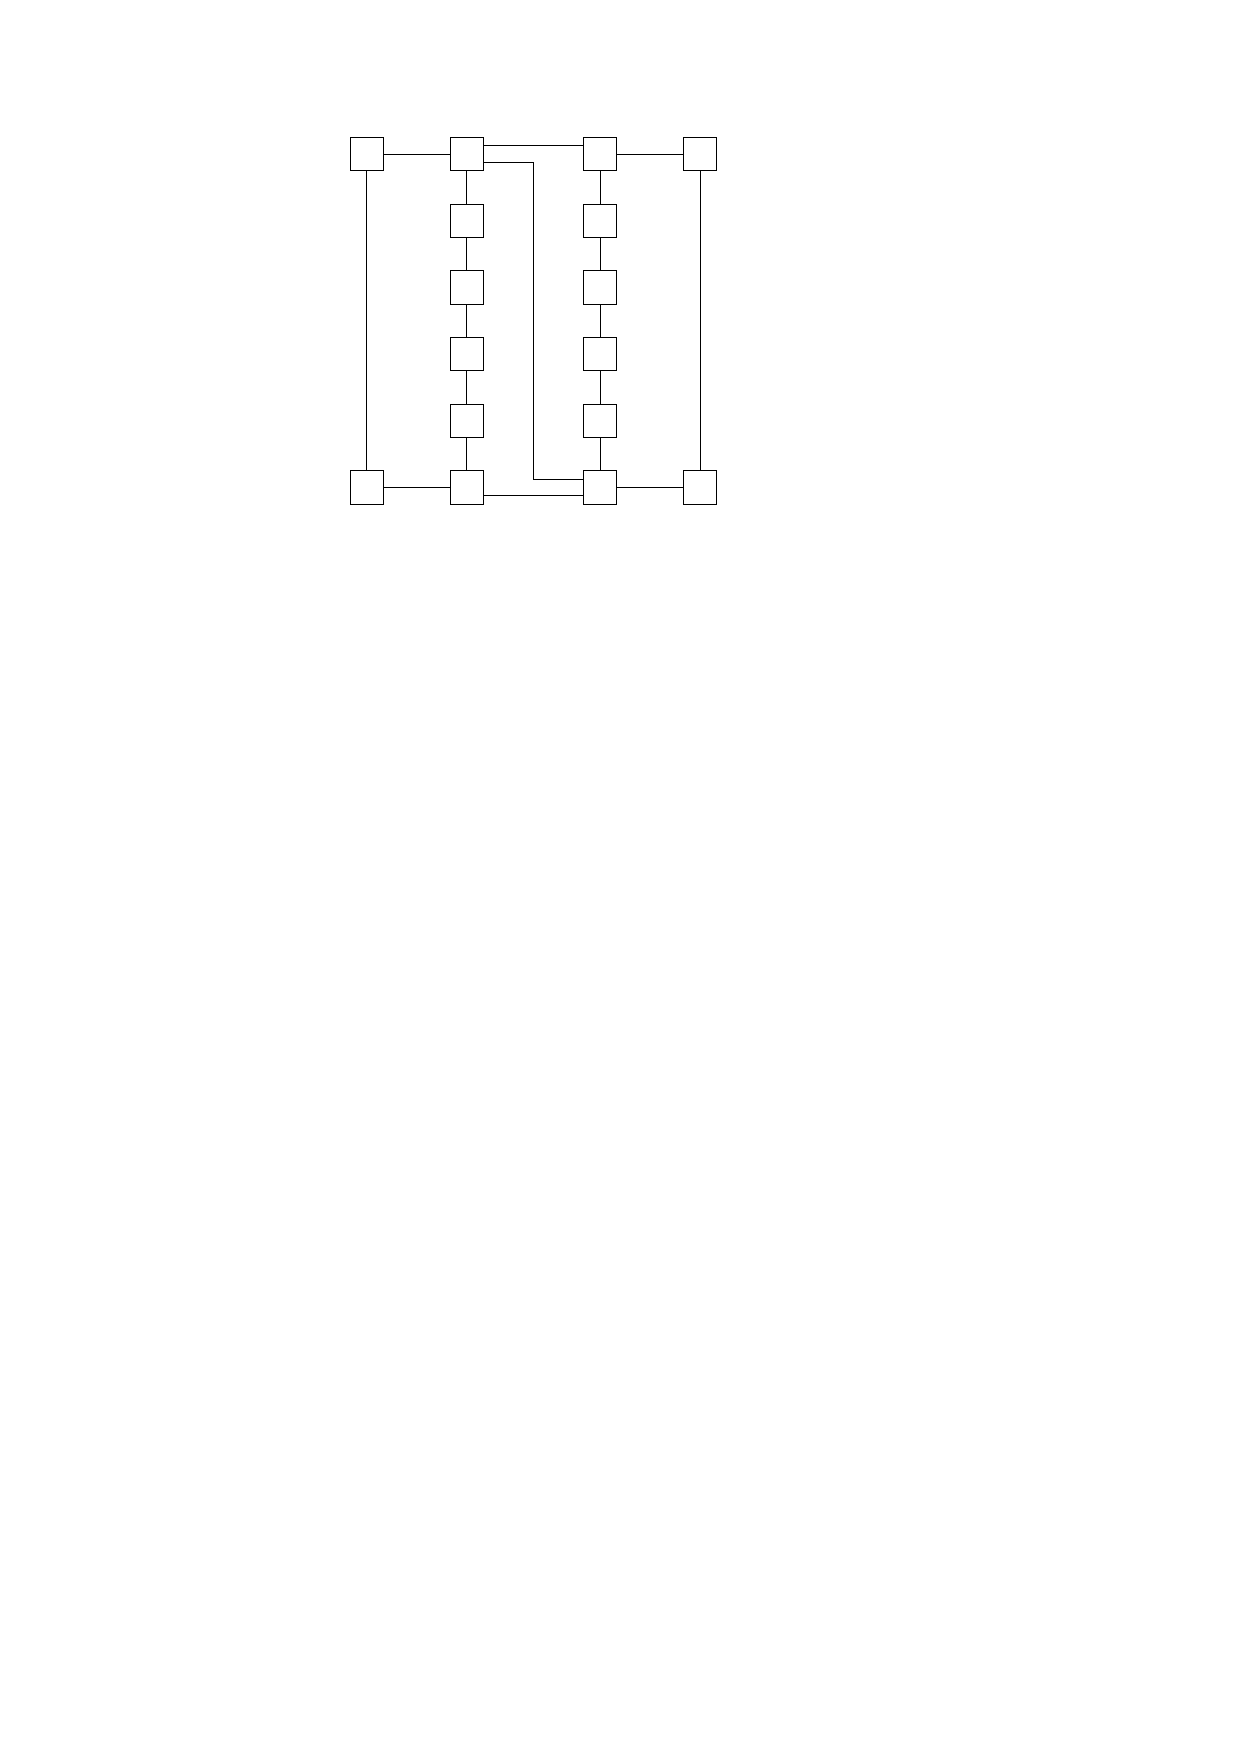
\includegraphics[width=0.45\textwidth,page=1]{includegraphics/port_reassignment_not_possible.pdf}
		\caption{}
	\end{subfigure}
	\begin{subfigure}{0.45\linewidth}
		\centering
		\includegraphics[width=0.7\textwidth,page=2]{includegraphics/port_reassignment_not_possible.pdf}
		\caption{}
	\end{subfigure}
	\caption{This might just be a candidate with negative result}\label{im:port_reassignment_not_possible}
\end{figure}
An approach to find candidate edges for a port reassignment could lie in \grqq half-bends\grqq~and diagonal segments, seen in the $L$ shape and the $T$ shape of the \textit{Kandinsky drawings with almost-empty faces} (Podevsaef drawings in short). In our first approach, we mainly focus on complexity-3 zig zags in the original Kandinsky Model.
\subsubsection{Podevsaef drawings}
Recalling definition \ref{def:podevsaef}, Podevsaef drawings mainly differ from SMOGs in their diagonal segments and 135\degree~bends. The approach to create a Podevsaef drawing is pretty similar to the smooth orthogonal case. At first, the planar Kandinsky drawing of the original graph $G$ is computed which then gets modified by a modification of the \textit{Topology Shape Metrics} algorithm (\cite[p. 4]{podevsaef}). The usage of diagonal segments enable us to illustrate triangular faces with two 135\degree~bends rather than 90\degree~bends. This solution for the bend or end property difficulty enables us to illustrate \textit{almost empty faces}, still inheriting bounding edges with a 0\degree~difference but not orthogonally, therefore \textit{almost} empty. The following solutions were found for $L$ shaped and $T$ shaped triangles:
\begin{figure}[H]
	\centering
	\begin{subfigure}{0.49\linewidth}
		\centering
		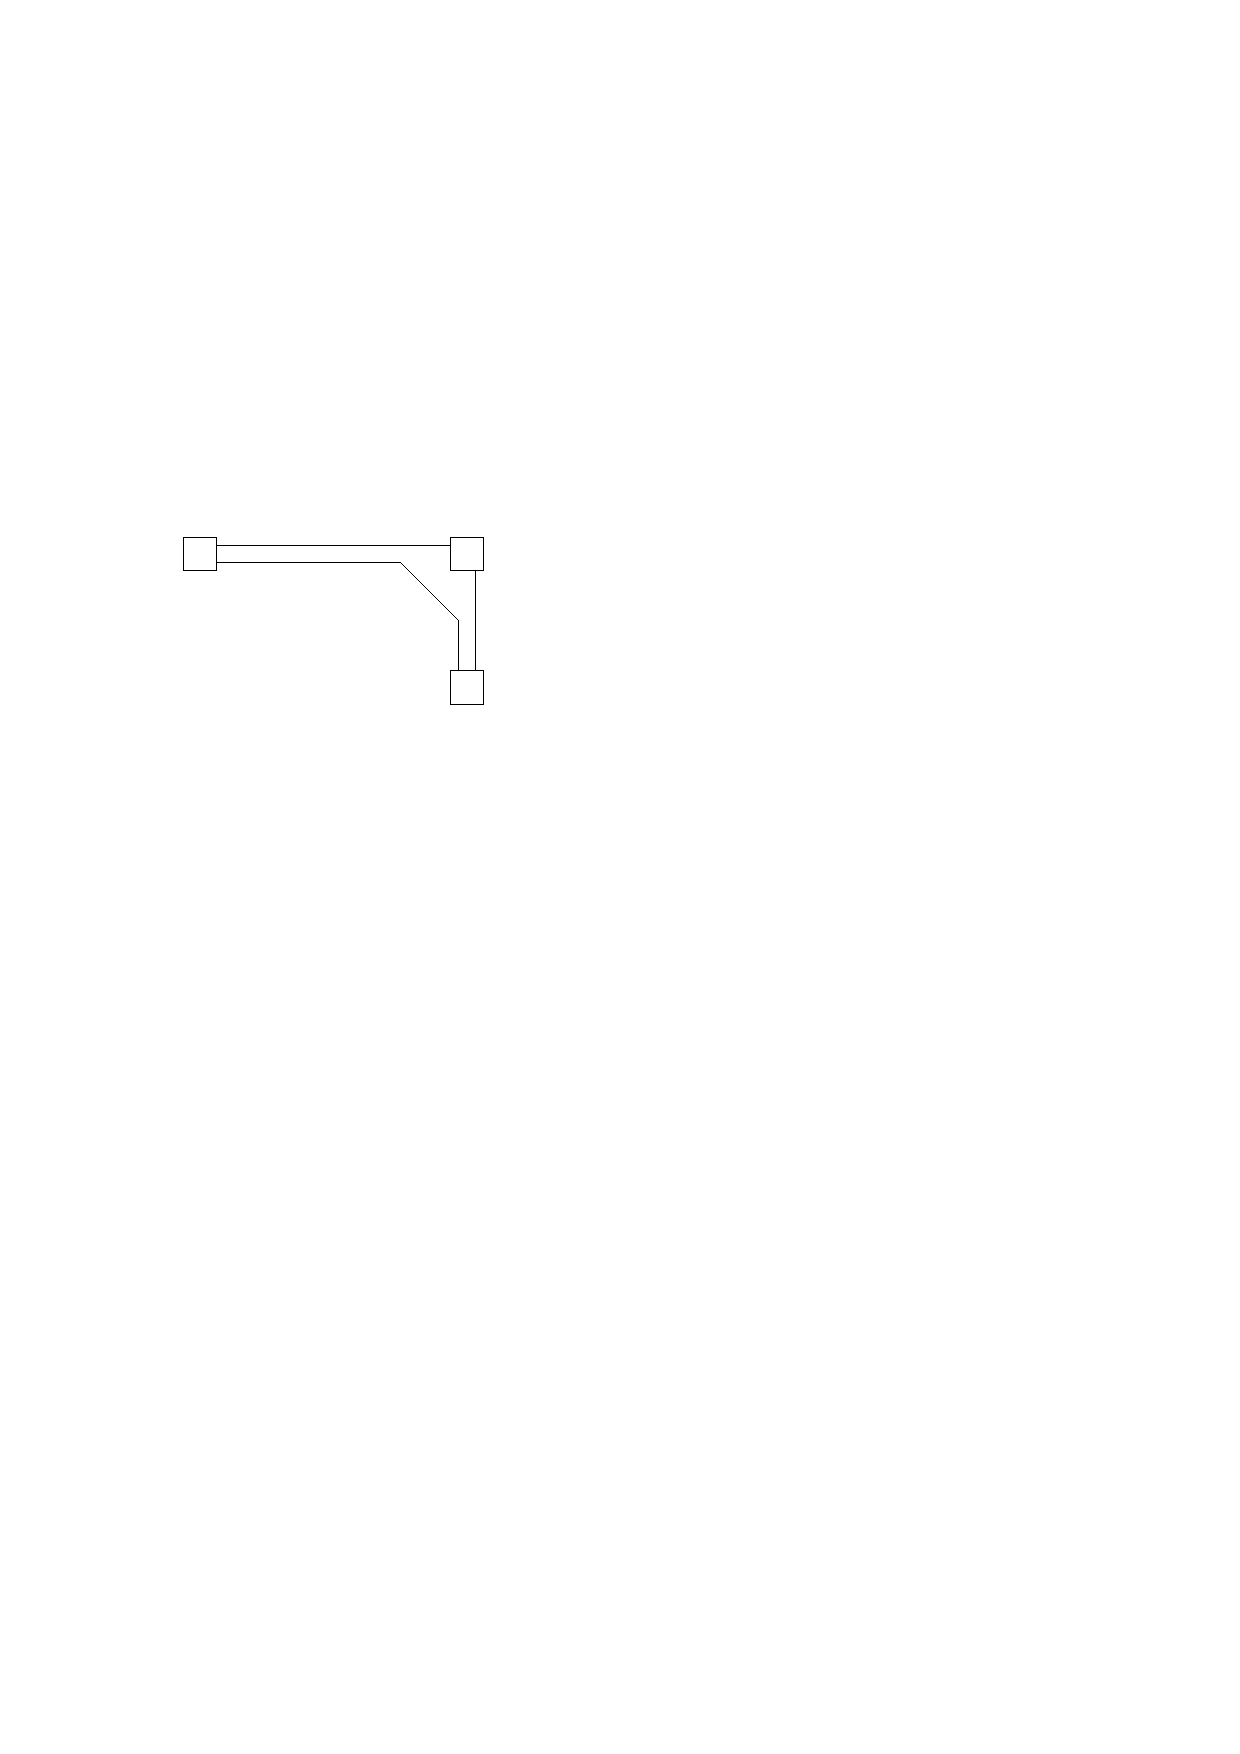
\includegraphics[width=0.471\textwidth,page=1]{includegraphics/L-t-shape_candidates.pdf}
		\caption{}
	\end{subfigure}
	\begin{subfigure}{0.49\linewidth}
		\centering
		\includegraphics[width=0.7\textwidth,page=2]{includegraphics/L-t-shape_candidates.pdf}
	\caption{}
\end{subfigure}
\caption{$L$ and $T$ shapes with almost empty faces}	
\end{figure}
Inspired by this illustration, we look for candidates for possible circular arc substitutions. Both examples from Figure \ref{im:recall1} and Figure \ref{im:port_reassignment_not_possible} might suit for a port reassignment. Although the complexity decrease possibility differs, they both share the achievable planar diagonal half-bend substitution after the application of the stretching technique.
\begin{figure}[H]
	\centering
	\begin{subfigure}{0.2\linewidth}
		\centering
		\includegraphics[width=0.8\textwidth,page=3]{includegraphics/L-t-shape_candidates.pdf}
		\caption{}\label{im:zig-zag_candidates1}
	\end{subfigure}
	\begin{subfigure}{0.39\linewidth}
		\centering
		\includegraphics[width=0.7\textwidth,page=4]{includegraphics/L-t-shape_candidates.pdf}
		\caption{}\label{im:zig-zag_candidates2}
	\end{subfigure}
	\begin{subfigure}{0.39\linewidth}
		\centering
		\includegraphics[width=0.7\textwidth,page=5]{includegraphics/L-t-shape_candidates.pdf}
		\caption{}\label{im:zig-zag_candidates3}
	\end{subfigure}
	\caption{Complexity-3 zig zags examined}\label{im:zig-zag_candidates}	
\end{figure}
\begin{lemma}If a polyedge representation $\Gamma_e$ is zig-zag shaped in Kandinsky (Figure \ref{im:zig-zag_candidates1}) and the port reassignment and circular arc substitution decrease the complexity in the resulting planar SMOG representation (Figure \ref{im:zig-zag_candidates2}), then there is a planar Podevsaef representation with two 135\degree~bends (Figure \ref{im:zig-zag_candidates3}).\label{lem:zig-zag_candidates}
\end{lemma}
So, according to lemma \ref{lem:zig-zag_candidates}, if we look for the possibility of planar Podevsaef polyedge representation like illustrated in figure \ref{im:zig-zag_candidates3} in a polyedge, the port reassignment of one of the vertices might just decrease the complexity. But as we seen, not in every case.
\subsubsection{Using the fragmentation}
Another approach is to use the optimal fragmentation regarding a polyedge to determine whether it was possible to save some bends. The fragmentation itself does not consider the horizontal or vertical alignment of segments in the plane. The following example will motivate the next lemma:
\begin{lemma}
	If the optimal fragmentation of a polyedge contains a fragment of length one in between two other fragments and its line segment is vertical, then the complexity does not increase at this incompatible fragment.
\end{lemma}
\begin{proof}
	Consider the alternating fragment consisting of a single vertical segment in the optimal fragmentation (Figure \ref{im:vertical_fragment2}). Then, the fragments adjacent to it are uniform. Those fragments share the same turn direction because in the uniform-only fragmentation the fragments are alternating their direction of turns. Consider that the original fragment was of length two without the recheck. The next fragment is of length at least three because the fragmentation algorithms have been shifting a second segment. This particular situation enables us to substitute the vertical segment with a half-circular arc due to the same turns of the segments before (Figure \ref{im:vertical_fragment3}). 
\begin{figure}[H]
	\centering
	\begin{subfigure}{0.33\linewidth}
		\centering
		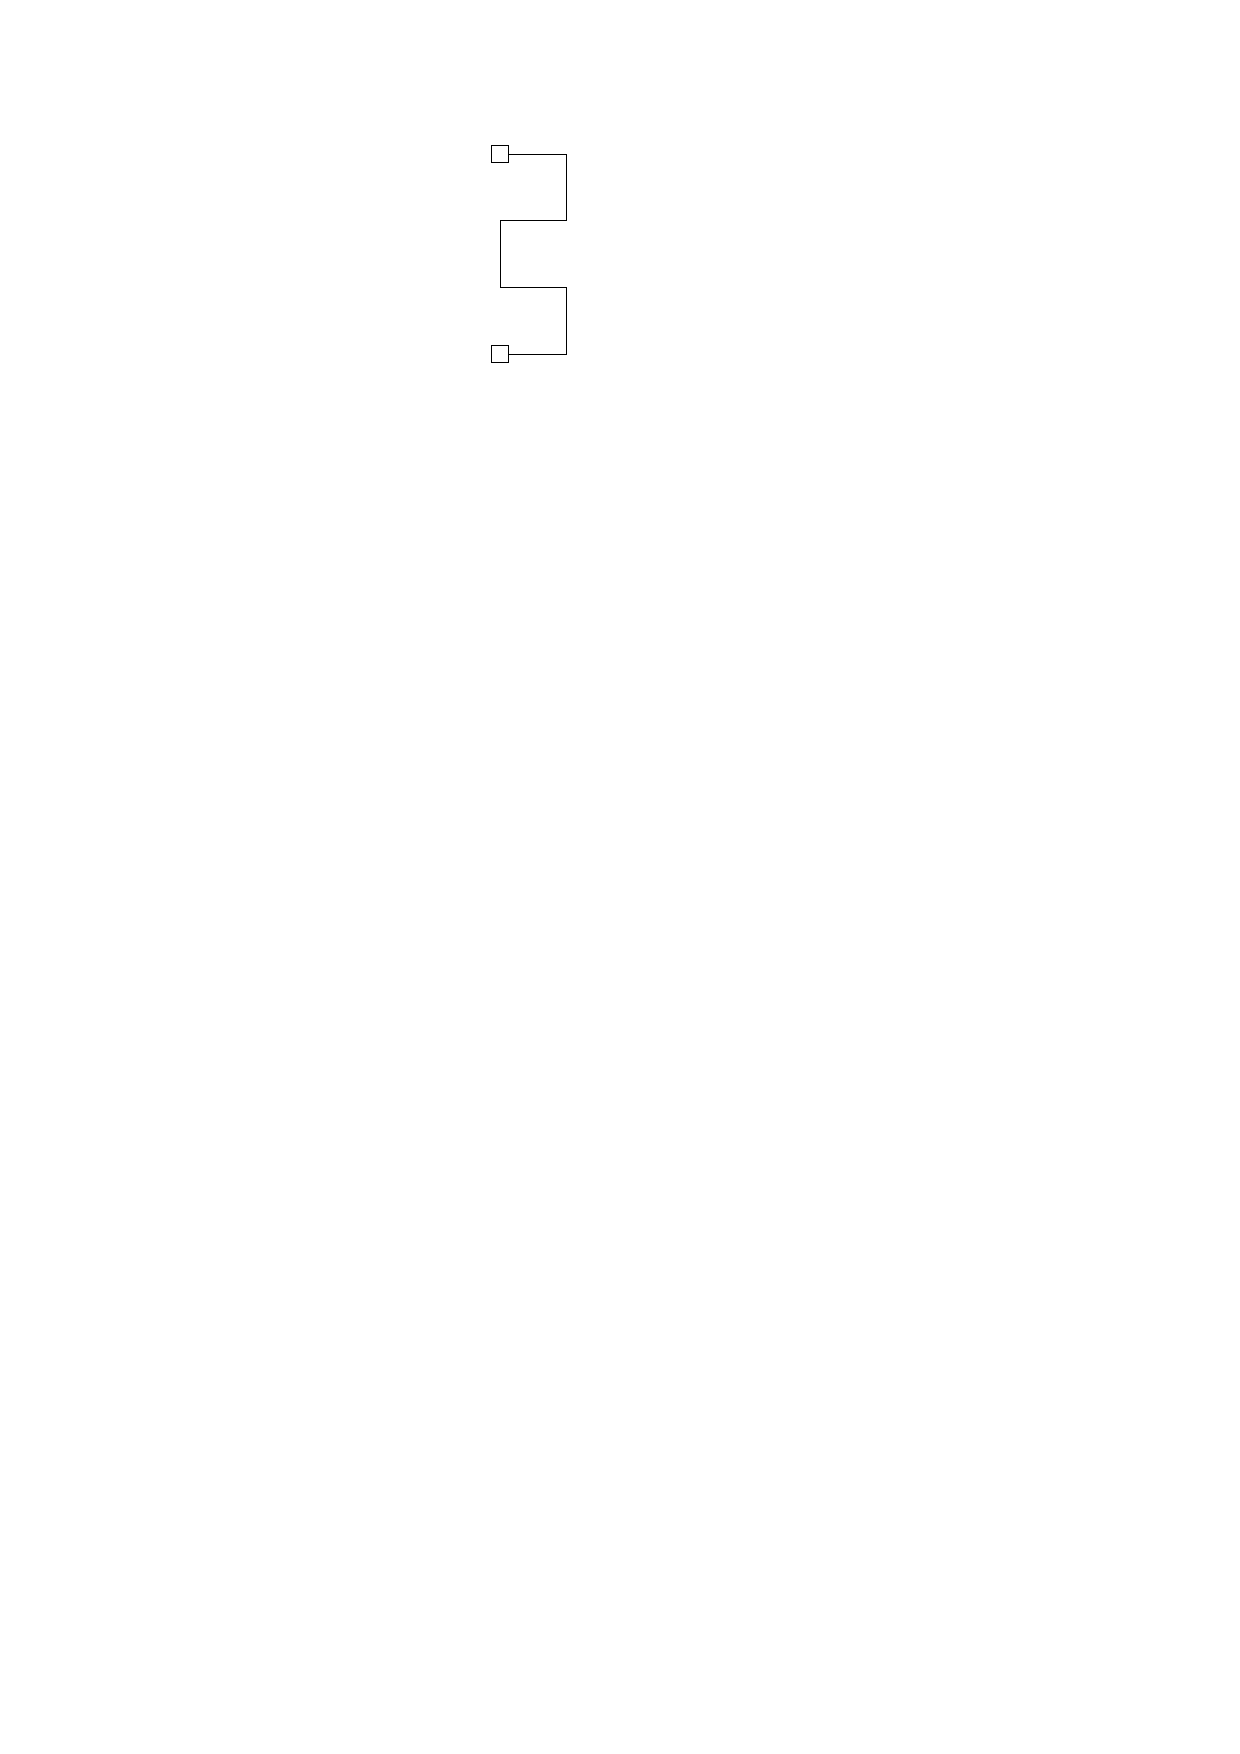
\includegraphics[width=0.25\textwidth,page=1]{includegraphics/vertical_fragment_1.pdf}
		\caption{}\label{im:vertical_fragment1}
	\end{subfigure}	
	\begin{subfigure}{0.33\linewidth}
		\centering
		\includegraphics[width=0.25\textwidth,page=2]{includegraphics/vertical_fragment_1.pdf}
		\caption{}\label{im:vertical_fragment2}
	\end{subfigure}
	\begin{subfigure}{0.32\linewidth}
		\centering
		\includegraphics[width=0.45\textwidth,page=3]{includegraphics/vertical_fragment_1.pdf}
		\caption{}\label{im:vertical_fragment3}
	\end{subfigure}
	\caption{Illustration of the alternating fragment exception}\label{im:vertical_fragment}
\end{figure}
\end{proof}
\subsection{Area Bounds}
In this section, we will examine the possiblities of area bound optimization. Suppose that the original orthogonal drawing is very large and contains a large number of vertices, it is of interest to find a way to lower the upper bound. In the first approach, we will erase redundancies in a drawing with a plane sweep method. In the second approach, we will substitute the circular arcs with ellipses or specific segment combinations in order to lower the upper bound by $\Rho(\sqrt{n})$, which may increase the lower bound of the edge complexity on the other hand.
\subsubsection*{Plane sweep erasing}
The stretching technique does not increase the edge complexity excessively. On the other hand, it may appear that the horizontal area expansion of a drawing is unnecessarily big. In this section, a linear runtime plane sweep may be a stable solution regarding area and even edge complexity retrenchment. Consider the following example:
\begin{figure}[H]
	\centering
	\begin{subfigure}{0.33\linewidth}
		\centering
		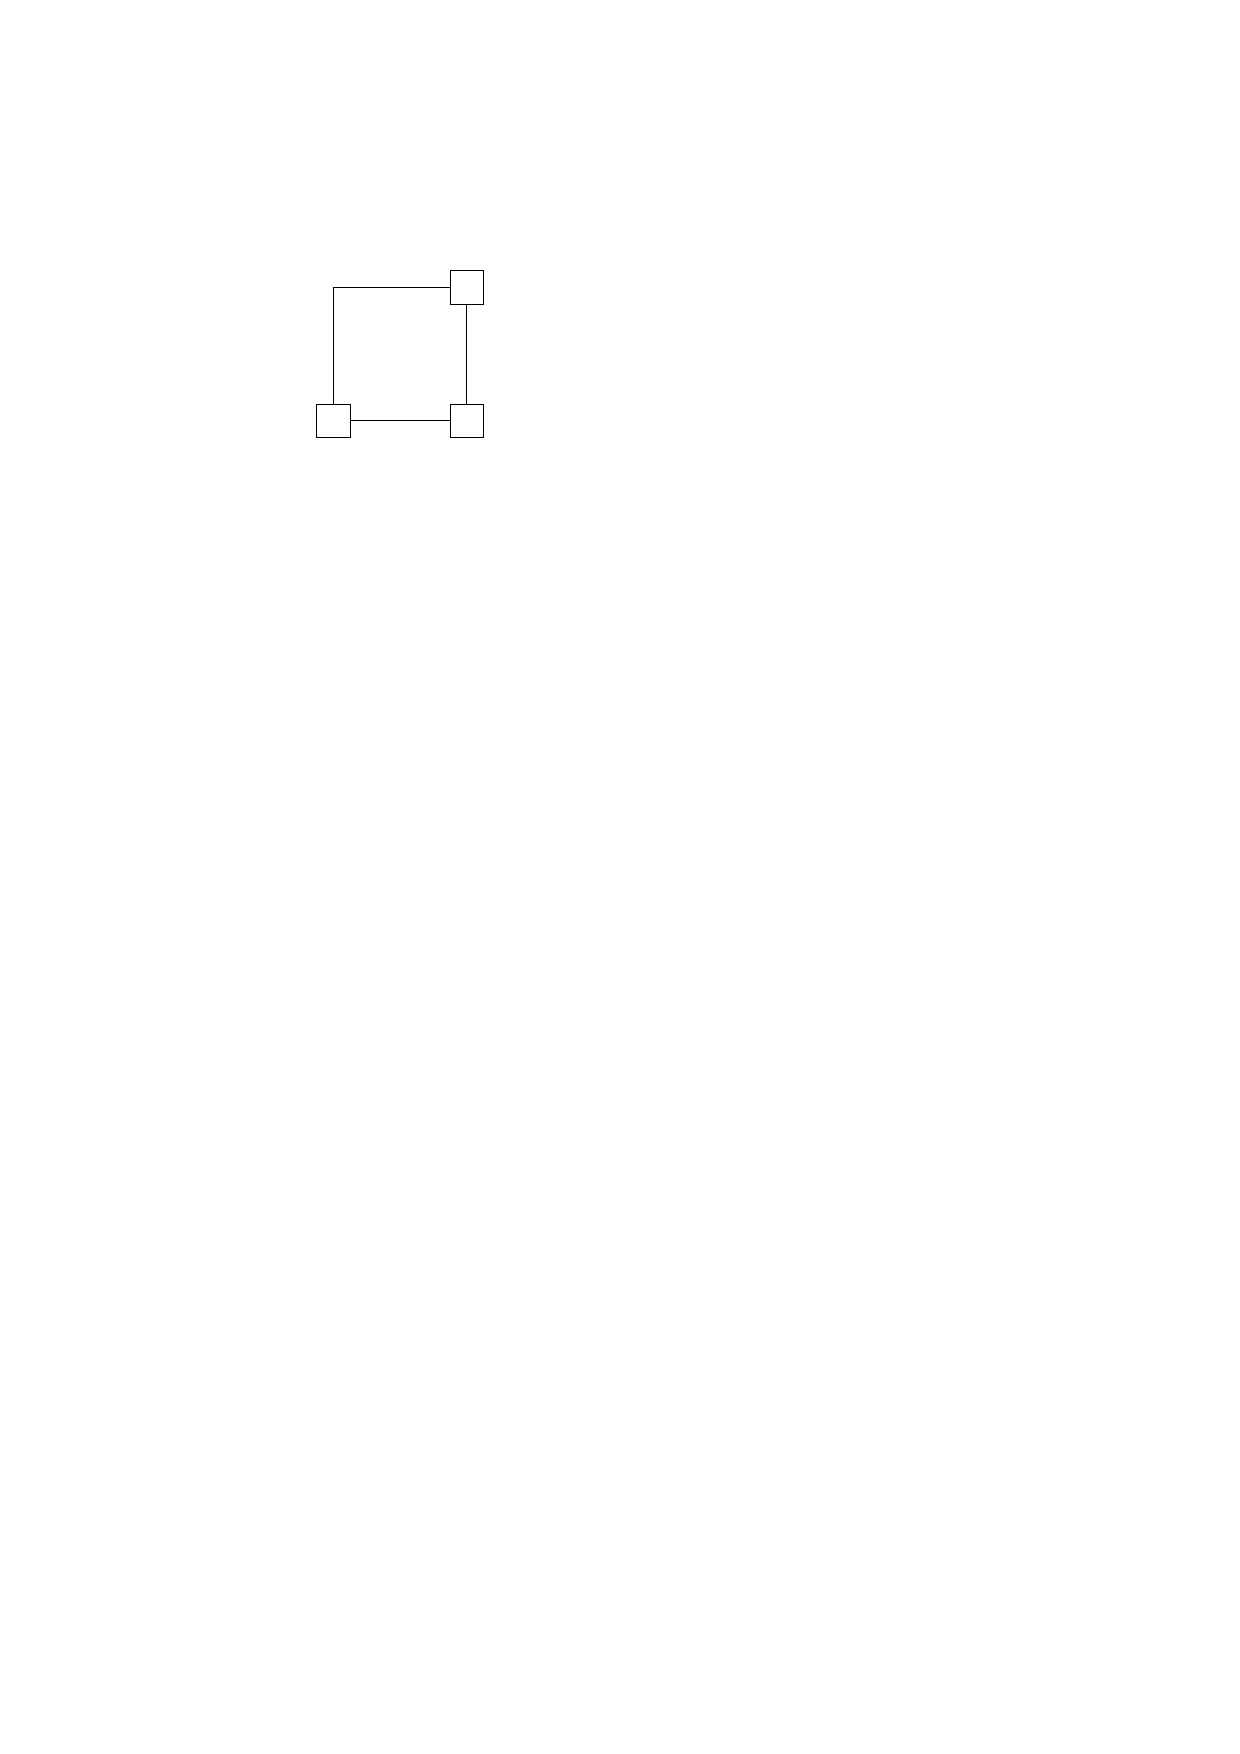
\includegraphics[width=0.4\textwidth,page=1]{includegraphics/plane_sweep_save.pdf}
		\caption{}
	\end{subfigure}	
	\begin{subfigure}{0.33\linewidth}
		\centering
		\includegraphics[width=0.8\textwidth,page=2]{includegraphics/plane_sweep_save.pdf}
		\caption{}
	\end{subfigure}
	\begin{subfigure}{0.32\linewidth}
		\centering
		\includegraphics[width=0.4\textwidth,page=3]{includegraphics/plane_sweep_save.pdf}
		\caption{}
	\end{subfigure}

	\caption{One plane sweep could eradicate redundant area and even segments without causing any damage}\label{im:sweep_save}
\end{figure}
As you can see in Figure \ref{im:sweep_save}, an orthogonal Kandinsky drawing of a triangle gets transferred to a smooth orthogonal drawing in the Fixed Shape Model. The vertical orange-colored lines show the possible saving of area. Even one horizontal segment is eliminated in the process, reducing the complexity of the drawing to one.
\begin{definition}
	There is a plane sweep algorithm which eliminates unnecessary space and may even save some segments in linear runtime regarding the size of the drawing. The vertical segments do not have to be considered by the plane sweep.
\end{definition}
This plane sweep algorithm identifies the presence of \textit{vertices} and \textit{circular arcs} as an event. Obviously, it is undesirable to interfere with circular arcs while cutting the drawing. First we show, that considering vertices, circular arcs and horizontal line segments is sufficient.\\
The \textit{vertical line segments} are not to be considered because either they end in one or two vertices. This means that vertices are sufficient in this case to be seen. If a vertical line segment is not connected to any vertex, then, by definition of the SMOG Model, they are connected to circular arcs which are also considered by the sweep line.\\
The horizontal segments are part of the events in order to determine which segments can be cut between two events. The plane sweep iterates from the left side to the right and is able to delete unnecessary horizontal redundancy with one sweep. Therefore, this plane sweep will run in linear runtime regarding the size of the drawing.
\begin{lemma}
	This area saving plane sweep is able to save up to $\Rho(\sqrt{w})$ area, where $w$ is the width of the input drawing and it potentially lowers the overall complexity of a drawing.
\end{lemma}
\begin{proof}
	Consider following orthogonal drawing of the graph:
	\begin{figure}[H]
		\centering
		\begin{subfigure}{0.45\linewidth}
			\centering
			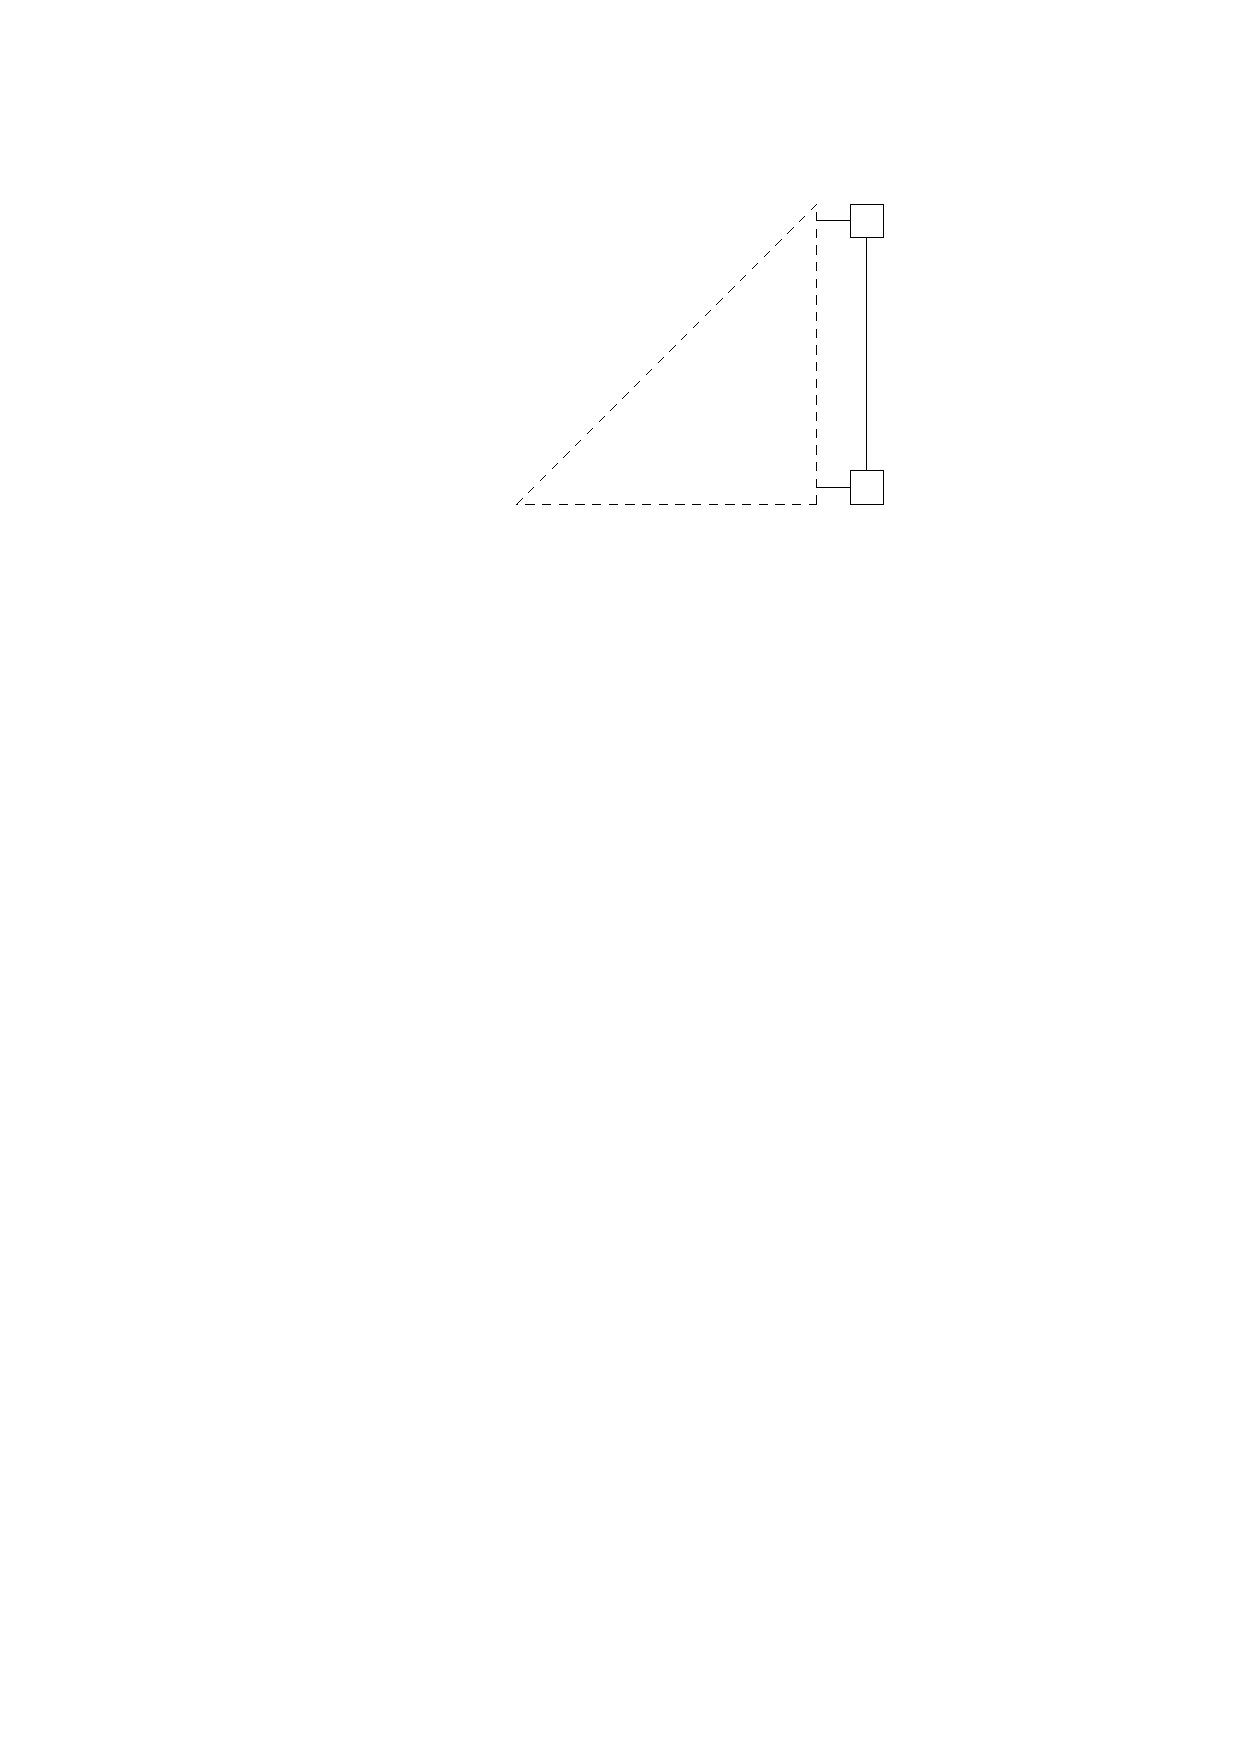
\includegraphics[width=0.5\textwidth,page=1]{includegraphics/plane_sweep_linear_saving.pdf}
			\caption{}\label{im:ortho_max_saving1}
		\end{subfigure}	
		\begin{subfigure}{0.4\linewidth}
			\centering
			\includegraphics[width=0.5\textwidth,page=2]{includegraphics/plane_sweep_linear_saving.pdf}
			\caption{}\label{im:ortho_max_saving2}
		\end{subfigure}
	\caption{Orthogonal drawing with maximal saving possibilites}\label{im:ortho_max_saving}
	\end{figure}
The dotted triangle of figure \ref{im:ortho_max_saving1} consists of $\Rho(n)\times\Rho(n)$ vertices as illustrated in figure \ref{im:ortho_max_saving2}. Applying the stretching technique and circular arc substitution, the resulting SMOG drawing is of size $\Rho(n^2)\times\Rho(n)$.
	\begin{figure}[H]
	\centering
	\begin{subfigure}{0.45\linewidth}
		\centering
		\includegraphics[width=0.7\textwidth,page=3]{includegraphics/plane_sweep_linear_saving.pdf}
		\caption{}\label{im:ortho_max_saving3}
	\end{subfigure}	
	\begin{subfigure}{0.4\linewidth}
		\centering
		\includegraphics[width=0.7\textwidth,page=4]{includegraphics/plane_sweep_linear_saving.pdf}
		\caption{}\label{im:ortho_max_saving4}
	\end{subfigure}
	\caption{SMOG drawing with maximal saving possibilites}
\end{figure}
In figure \ref{im:ortho_max_saving4}, the orange dotted lines indicate where the area saving plane sweep triggers an event. Notice that there are $\Rho(n)$ events.
	\begin{figure}[H]
	\centering
	\begin{subfigure}{0.45\linewidth}
		\centering
		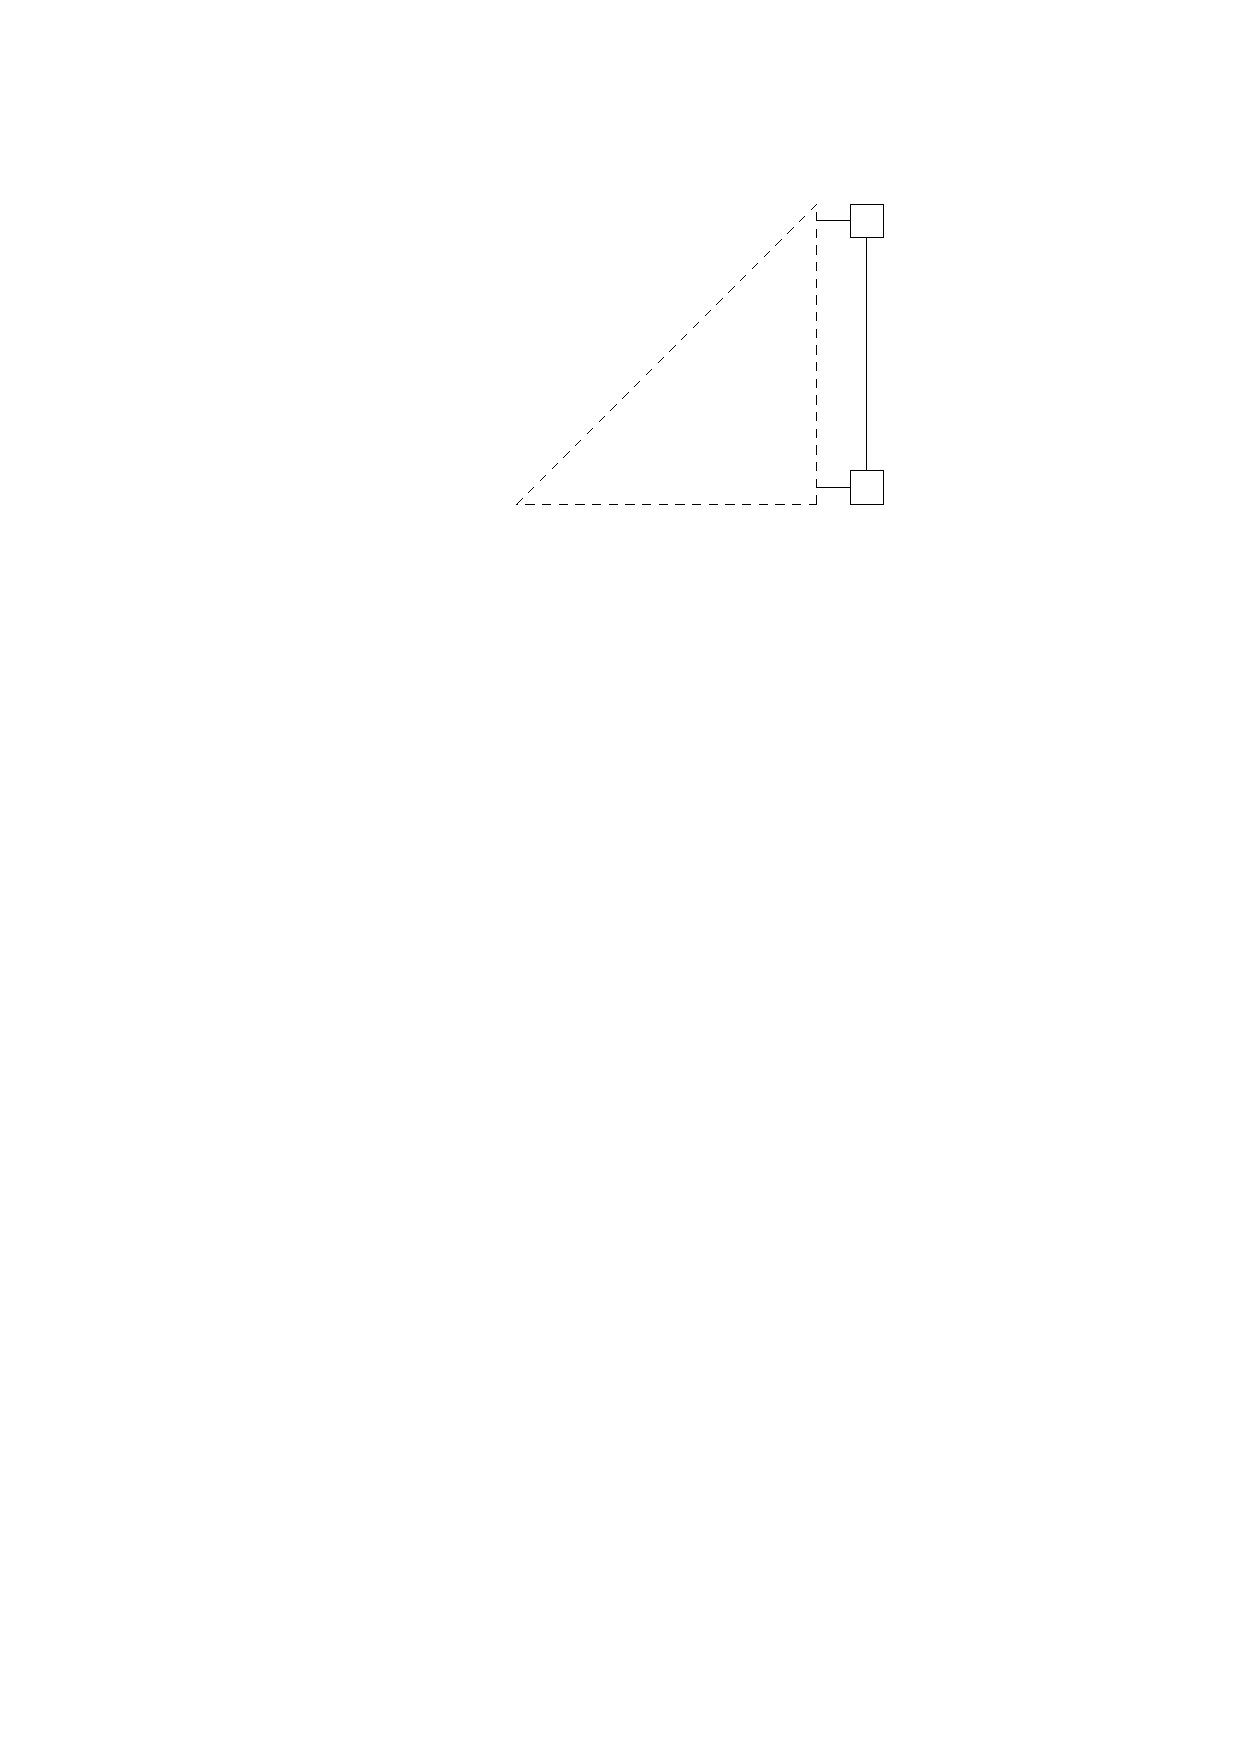
\includegraphics[width=0.5\textwidth,page=1]{includegraphics/plane_sweep_linear_saving.pdf}
		\caption{}
	\end{subfigure}	
	\begin{subfigure}{0.4\linewidth}
		\centering
		\includegraphics[width=0.5\textwidth,page=5]{includegraphics/plane_sweep_linear_saving.pdf}
		\caption{}\label{im:ortho_max_saving5}
	\end{subfigure}
	\caption{SMOG drawing after applying the plane sweep}
\end{figure}
After cutting area redundancies, we decrease the complexity of the graph to one and save $\Rho(n)$ area horizontally.
\end{proof}
However, the plane sweep will not work properly in all scenarios, as the following example will show:
\begin{figure}[H]
	\centering
	\begin{subfigure}{0.5\linewidth}
		\centering
		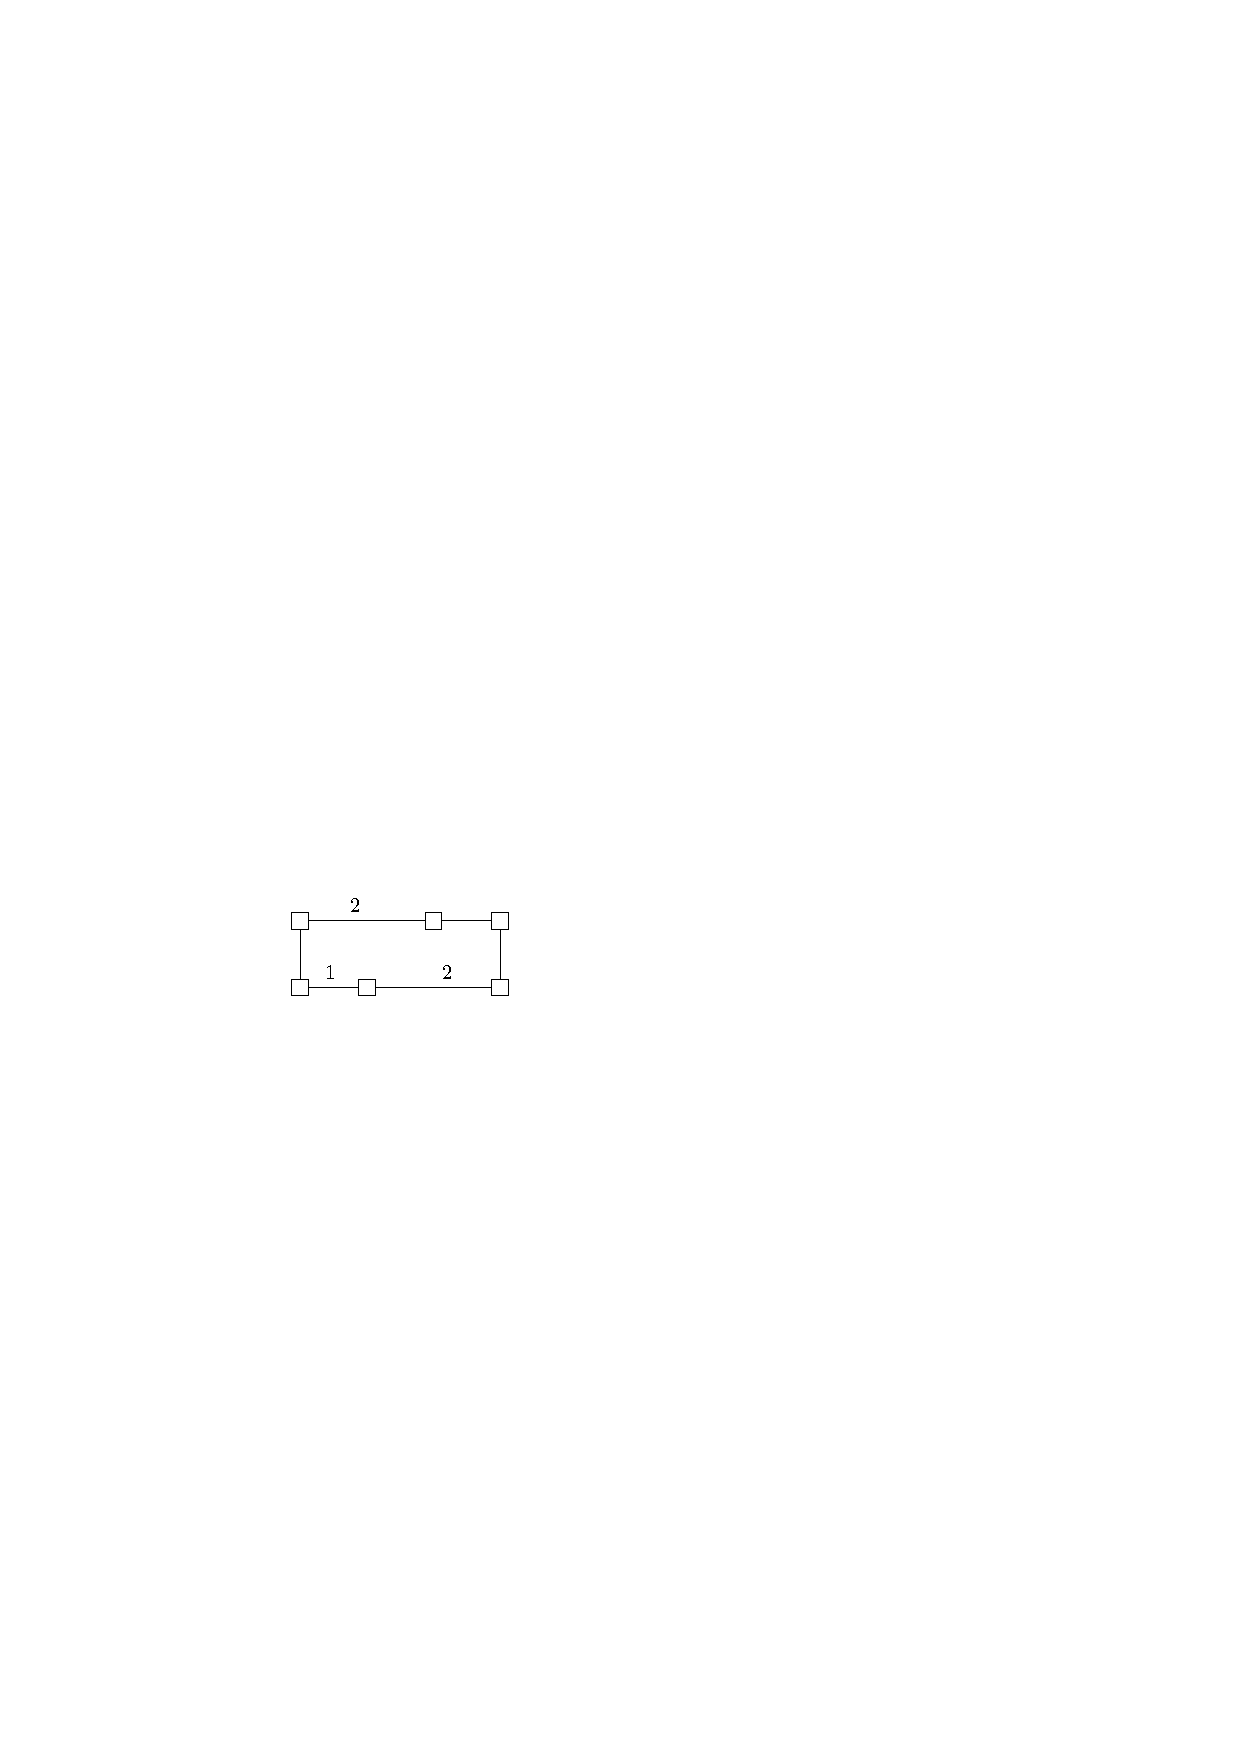
\includegraphics[width=0.6\textwidth,page=1]{includegraphics/plane_sweep_not_working.pdf}
	\end{subfigure}
	\caption{The plane sweep will not reduce anything}\label{im:plane_sweep_bad_example1}
\end{figure}
Consider the drawing in Figure \ref{im:plane_sweep_bad_example1} with a unit length of 1. While iterating from left to right, there will be a vertex as a new event with unit length difference to the last event. However, this drawing can be optimized regarding horizontal area as shown in figure \ref{im:plane_sweep_bad_example2}.
\begin{figure}[H]
	\centering
	\begin{subfigure}{0.5\linewidth}
		\centering
		\includegraphics[width=0.6\textwidth,page=2]{includegraphics/plane_sweep_not_working.pdf}
	\end{subfigure}
	\caption{Optimized drawing derived from figure \ref{im:plane_sweep_bad_example1}}
	\label{im:plane_sweep_bad_example2}
\end{figure}
In order to find a solution for this situation, a new approach based on the \textit{4M} algorithm is formulated.
\subsubsection{Modified 4M - Moving}
Recalling section \ref{section:4M}, the 4M algorithm consists of multiple operations. In this section, we will consider the \textit{moving} operation. 
\subsubsection*{Model consistency}
It is to examine whether the \textit{4M} operations were suitable for drawings which underly the Kandinsky model. In the Kandinsky model, the vertices are represented with boxes of uniform size. In the orthogonal 4M model, the boxes have to overlap the grid lines by $\frac{\lambda}{4}$, and the rectangles were of size $\left(w\lambda-\frac{\lambda}{2} \right)\times \left( h\lambda-\frac{\lambda}{2}\right);w,h\in\mathbb{N}$. By setting $w = h = 1$, we achieve a consistency with the Kandinsky model and therefore can continue examining a 4M algorithm modification.
\subsubsection*{The modification}
The focus lies in the horizontal area saving. The moving line $J$ will still be directed and starts above to topmost object and ends below the bottommost object of the drawing. Considering orthogonal graphs, $J$ only crosses horizontal lines from top to bottom. In the smoothened Kandinsky case, quarter circular arcs traverse in height and width - so they also have to be crossed for total area savings. 
\begin{figure}[H]
	\centering
	\begin{subfigure}{0.4\linewidth}
		\centering
		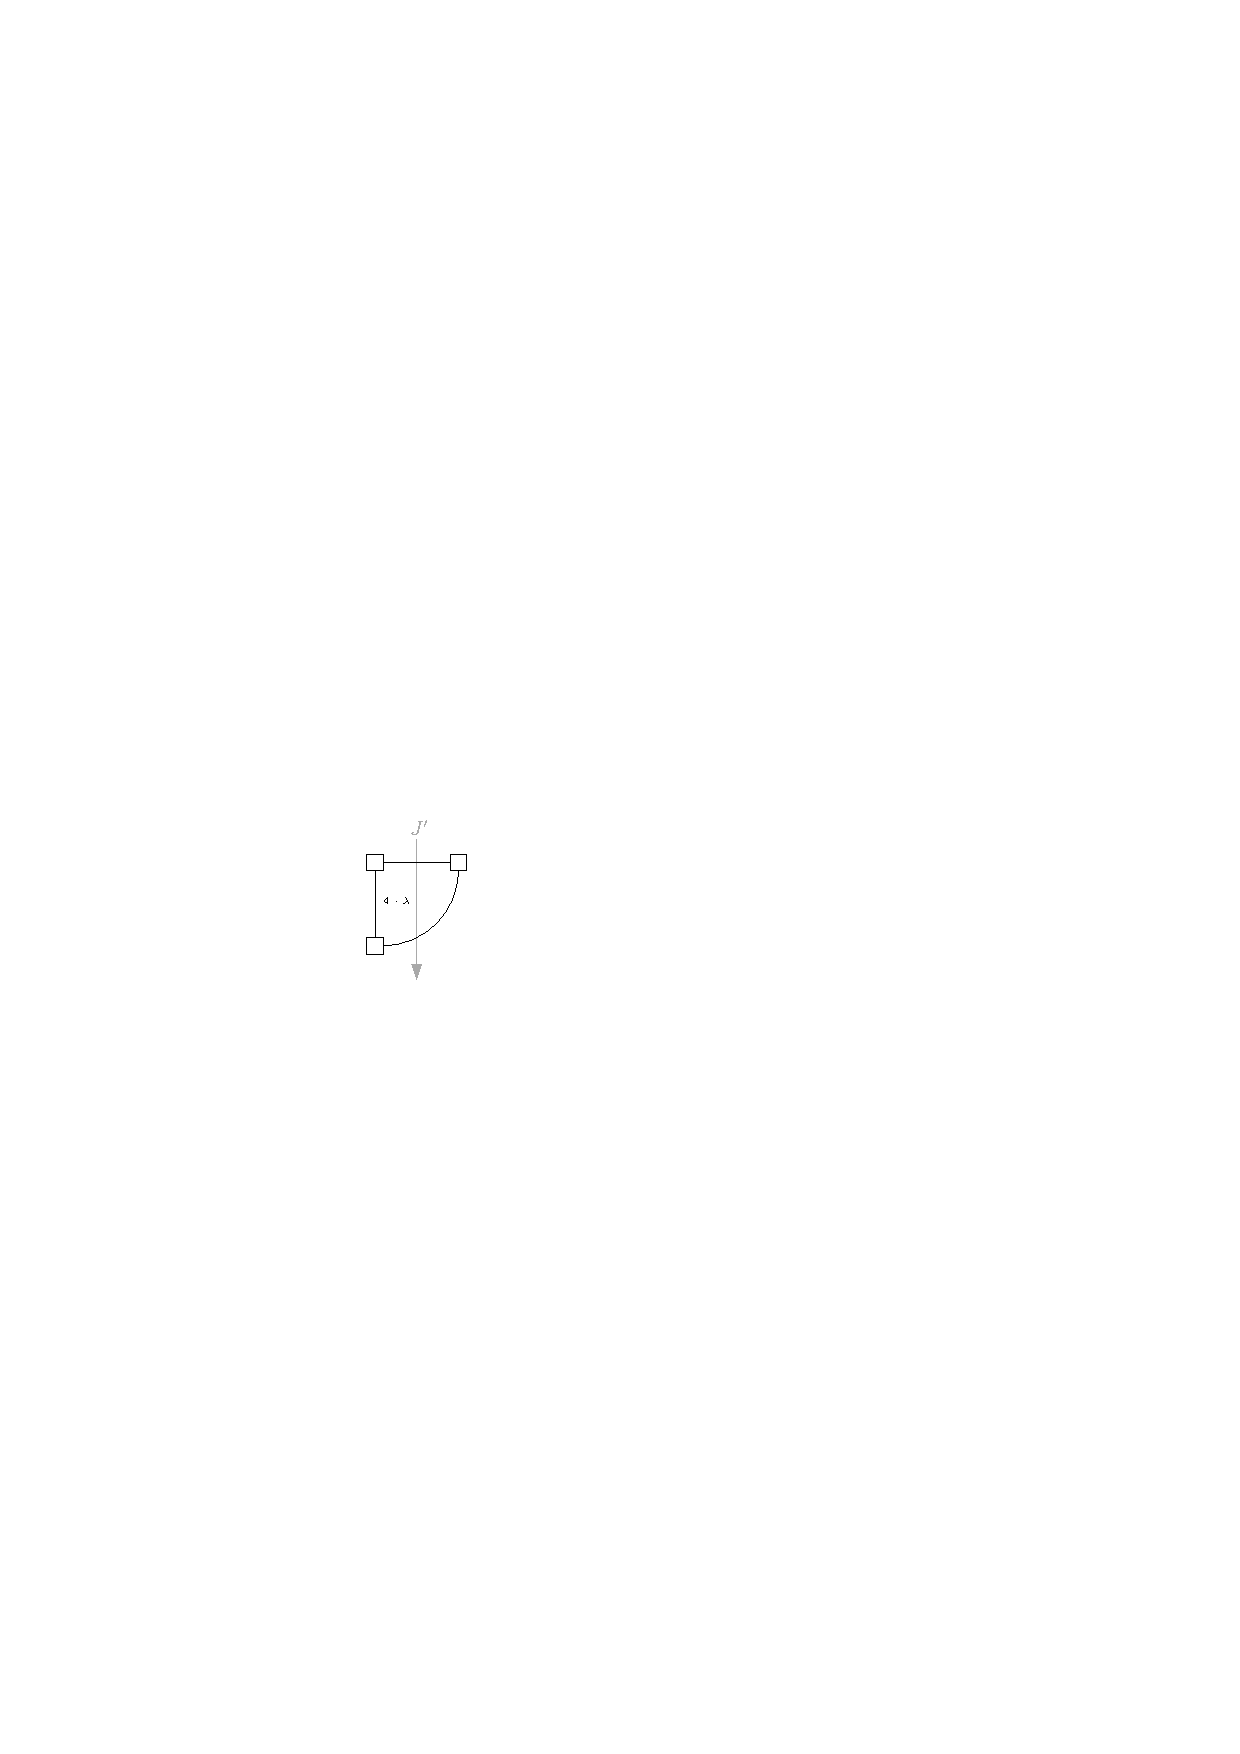
\includegraphics[width=0.4\textwidth,page=1]{includegraphics/4M_Moving_arcs.pdf}
		\caption{$J$ crossing the drawing}
	\end{subfigure}
	\begin{subfigure}{0.4\linewidth}
		\centering
		\includegraphics[width=0.2\textwidth,page=2]{includegraphics/4M_Moving_arcs.pdf}
		\caption{Circular arc substitution}
	\end{subfigure}
	\caption{A first, easy example}\label{im:arc-crossing_example1}
\end{figure}
As you can see in figure \ref{im:arc-crossing_example1}, a quarter circular arc with radius $r$ can be reduced in width by substituting with a circular arc with radius $r-c\cdot\lambda$ and a vertical segment of length $c\cdot\lambda$. $\lambda$ describes the unit length, $c$ describes the amount of unit reducings possible along $J$. By this method, the complexity may increase by one per crossed quarter circular arc. 
\begin{figure}[H]
	\centering
	\begin{subfigure}{0.4\linewidth}
		\centering
		\includegraphics[width=0.4\textwidth,page=3]{includegraphics/4M_Moving_arcs.pdf}
		\caption{$J'$ crossing the drawing}\label{im:arc-crossing_example2a}
	\end{subfigure}
	\begin{subfigure}{0.4\linewidth}
		\centering
		\includegraphics[width=0.265\textwidth,page=4]{includegraphics/4M_Moving_arcs.pdf}
		\caption{Quarter circular arc substitution}
	\end{subfigure}
	\caption{A second example}\label{im:arc-crossing_example2}
\end{figure}
In this example, $J'$ crosses two consecutive quarter circular arcs in a drawing of size $6\times6$. The result is a drawing of size $4\times6$, with an edge complexity of three. A verticel line segment of length one is introduced per substituted arc, merged to a vertical line segment of length two.\\
To further decrease the area of the drawing, a horizontal path from the leftmost object to the rightmost one would reduce and even eliminate the vertical line segments crossed by $J'$.
\begin{figure}[H]
	\centering
	\begin{subfigure}{0.4\linewidth}
		\centering
		\includegraphics[width=0.7\textwidth,page=5]{includegraphics/4M_Moving_arcs.pdf}
		\caption{$J'$ crossing the drawing}
	\end{subfigure}
	\begin{subfigure}{0.4\linewidth}
		\centering
		\includegraphics[width=0.7\textwidth,page=6]{includegraphics/4M_Moving_arcs.pdf}
		\caption{Circular arc substitution}
	\end{subfigure}
	\caption{Vertical area saving}\label{im:arc-crossing_example3}
\end{figure}
The area bounds of the drawing from Figure \ref{im:arc-crossing_example2a} can further be reduced by a horizontal moving line $J'$, resulting in a $4\times4$ drawing. In order to do so, one has to \textit{reduce the line segment between quarter circular arcs first}. This results in a possible complexity decrease, in this case a drawing of complexity two. \\
Recall the elongation of horizontal edges crossed by the original moving line $J$ with an upward direction. What, if a quarter circular arc is crossed with an upward piece of $J'$? Then, the idea is to add a horizontal line to the quarter circular arc correspondingly with unit length. Consider the following example:
\begin{figure}[H]
	\centering
		\begin{subfigure}{0.4\linewidth}
		\centering
		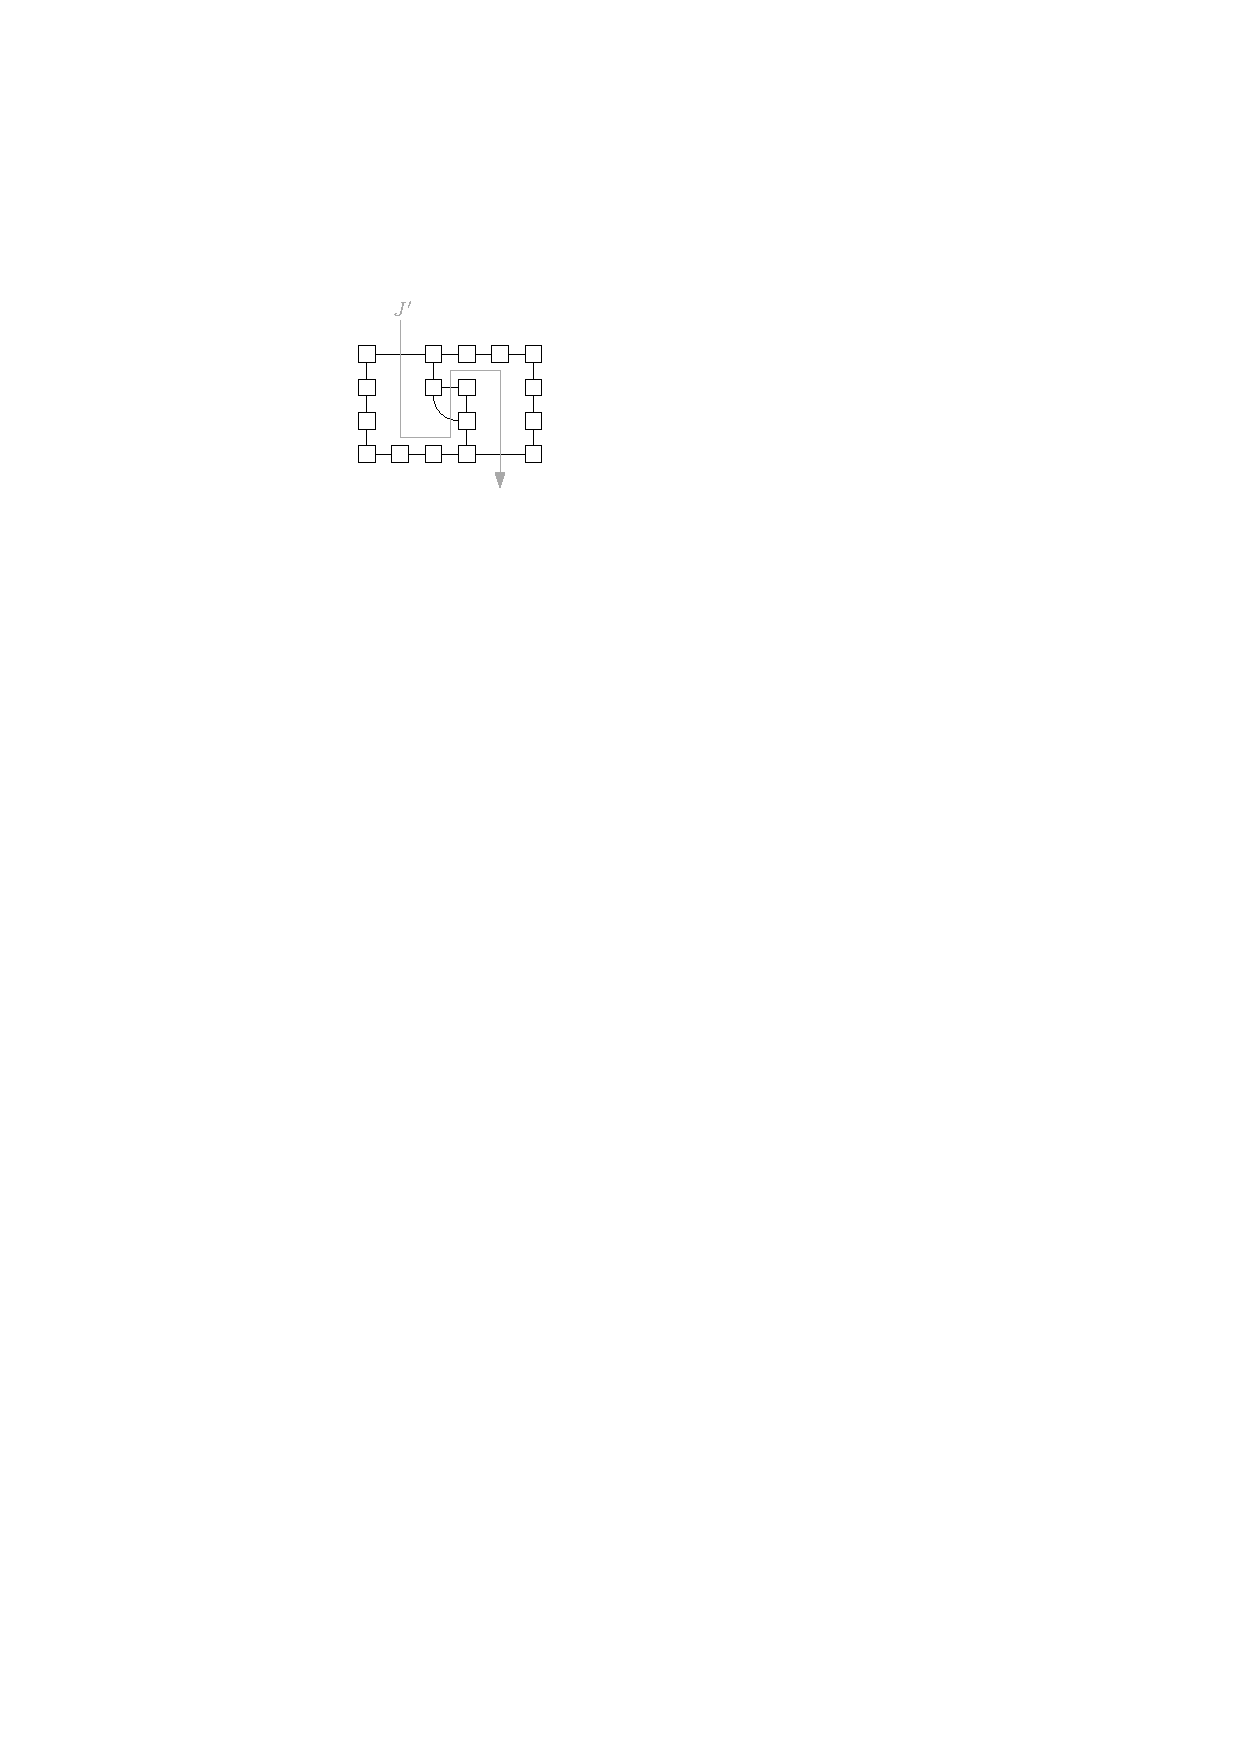
\includegraphics[width=0.7\textwidth,page=1]{includegraphics/4M_Moving_arcs_upward.pdf}
		\caption{$J'$ crossing the drawing}
	\end{subfigure}
	\begin{subfigure}{0.4\linewidth}
		\centering
		\includegraphics[width=0.6\textwidth,page=2]{includegraphics/4M_Moving_arcs_upward.pdf}
		\caption{Additional horizontal segments}
	\end{subfigure}
	\caption{The additional horizontal line segment increases the complexity of the drawing to two}
\end{figure}
This idea implies the modified moving approach.
\begin{definition}[modified moving line $J'$]
	An area-saving moving line $J'$ for a smoothened drawing $\Gamma ''$ is a line that fulfills the following conditions:
	\begin{itemize}
		\item $J'$ is directed and consists of horizontal and vertical segments
		\item $J'$ starts above the topmost object of $\Gamma ''$ and ends below the bottommost object of $\Gamma ''$
		\item $J'$ does not intersect any vertical edge of $\Gamma ''$
		\item In a polyedge $e$, either quarter circular arc segments or horizontal line segments might be crossed by $J'$ 
		\item Every horizontal edge of $\Gamma''$ that is intersected by a piece of $J'$ which is directed downward has a finite length larger than or equal to two. If this horizontal line segment is connected to a circular arc segment, then it has a finite length larger or equal to one.
		\item Every circular arc segment of $\Gamma''$ that is intersected by a piece of $J'$ which is directed downward has a finite radius larger than or equal to two.
	\end{itemize}
\end{definition}
Since $\Gamma''$ is planar, its dual graph is well-defined and planar. $J'$ can easily be found with \textit{depth first search} in the planar dual graph. 
Then, after finding $J'$, a smaller drawing can be computed the following way:
\begin{itemize}
	\item The length of every edge of $\Gamma''$ that is crossed by $J'$ in downward direction is decreased by one unit
	\item Simultaneously, the length of every edge crossed by $J'$ in upward direction is increased by one unit
	\item If a quarter circular arc is crossed by $J'$ in downward direction, then the arc is substituted by a quarter circular arc with a smaller radius by one unit with a vertical segment of unit length (refer to Figure \ref{im:arc-crossing_example1})
	\item If a quarter circular arc is crossed by $J'$ in upward direction, then a horizontal line segment of unit length is appended to the quarter circular arc correspondingly
\end{itemize}
Note, that this modified moving algorithm separates the drawing in two parts according to $J'$ and then moving one part closer to the other one. The direction of area saving can be altered by switching the roles of vertical and horizontal line segments and finding a horizontal directed path $J'$ instead of a vertical one.
\subsubsection*{Correctness}
Consider a quarter circular arc $c$ with radius $r$ crossed by $J'$ in a smoothened drawing. By substituting $c$ with a corresponding horizontal and vertical line segment, $h_c$ and $v_c$ with length $r$, the original moving algorithm preserves the planarity of the drawing.
\\
If the original moving line $J$ crosses $h_c$ downwards, then $h_c$ will be shorter in length than $v_c$. The substitution with a smaller circular arc with radius $|h_c|$ will increase the total edge complexity since $|v_c| > |h_c|$.
\\If the original moving line $J$ crosses $h_c$ upwards, then $h_c$ will be larger in length than $v_c$. The substitution with the input circular arc with radius $|v_c|$ increases the complexity since $|v_c| < |h_c|$. 
\\The area necessary for circular arc substitution is already proven in the previous section, preserving the planarity.
\\All we need to prove is the choice of segment to cross, when a horizontal line segment $h$ is appended to a circular arc $c$. We will be able to reduce $h$ successively until $h$ may be completely erased because $c$ is still unaltered and travels the width and height necessary for the drawing. Thus, we will choose $h$ for being crossed by $J'$, possibly achieving an edge complexity reduction.
\subsubsection{Circular arc substitution}
The circular arcs used in smooth orthogonal drawings have a height and width of $r$ and are the main reason for the quadratic total width in the worst case. In this section, we examine the possibilites of saving some space by substituting the circular arcs used with different segments. In our first approach, we will use ellipses to guarantee a width of $\sqrt{r}$, saving at least $\sqrt{n}$ area requirements. However, the aesthetics may suffer for large values. In our second approach, we will substitute the circular arc with a combination of a smaller circular arc and a vertical segment, also demanding $\sqrt{r}$ width. The aesthetics may be preserved but this definitely will increase the edge complexity of any drawing.
\subsubsection*{Ellipses}
Using a quarter of an ellipse, we could achieve a guaranteed width of $\sqrt{r}$, resulting in drawings of size $\Rho(n\cdot\sqrt{n})\times\Rho(n)$. We will take a look at following example equation given for an ellipse:
\begin{align}
\frac{x^2}{5} + \frac{y^2}{25} = 1&&x,-y \in \mathbb{R}_+\label{eq:ellipse_example}
\end{align}
\begin{figure}[H]
	\centering
	\begin{subfigure}{0.4\textwidth}
		\centering
		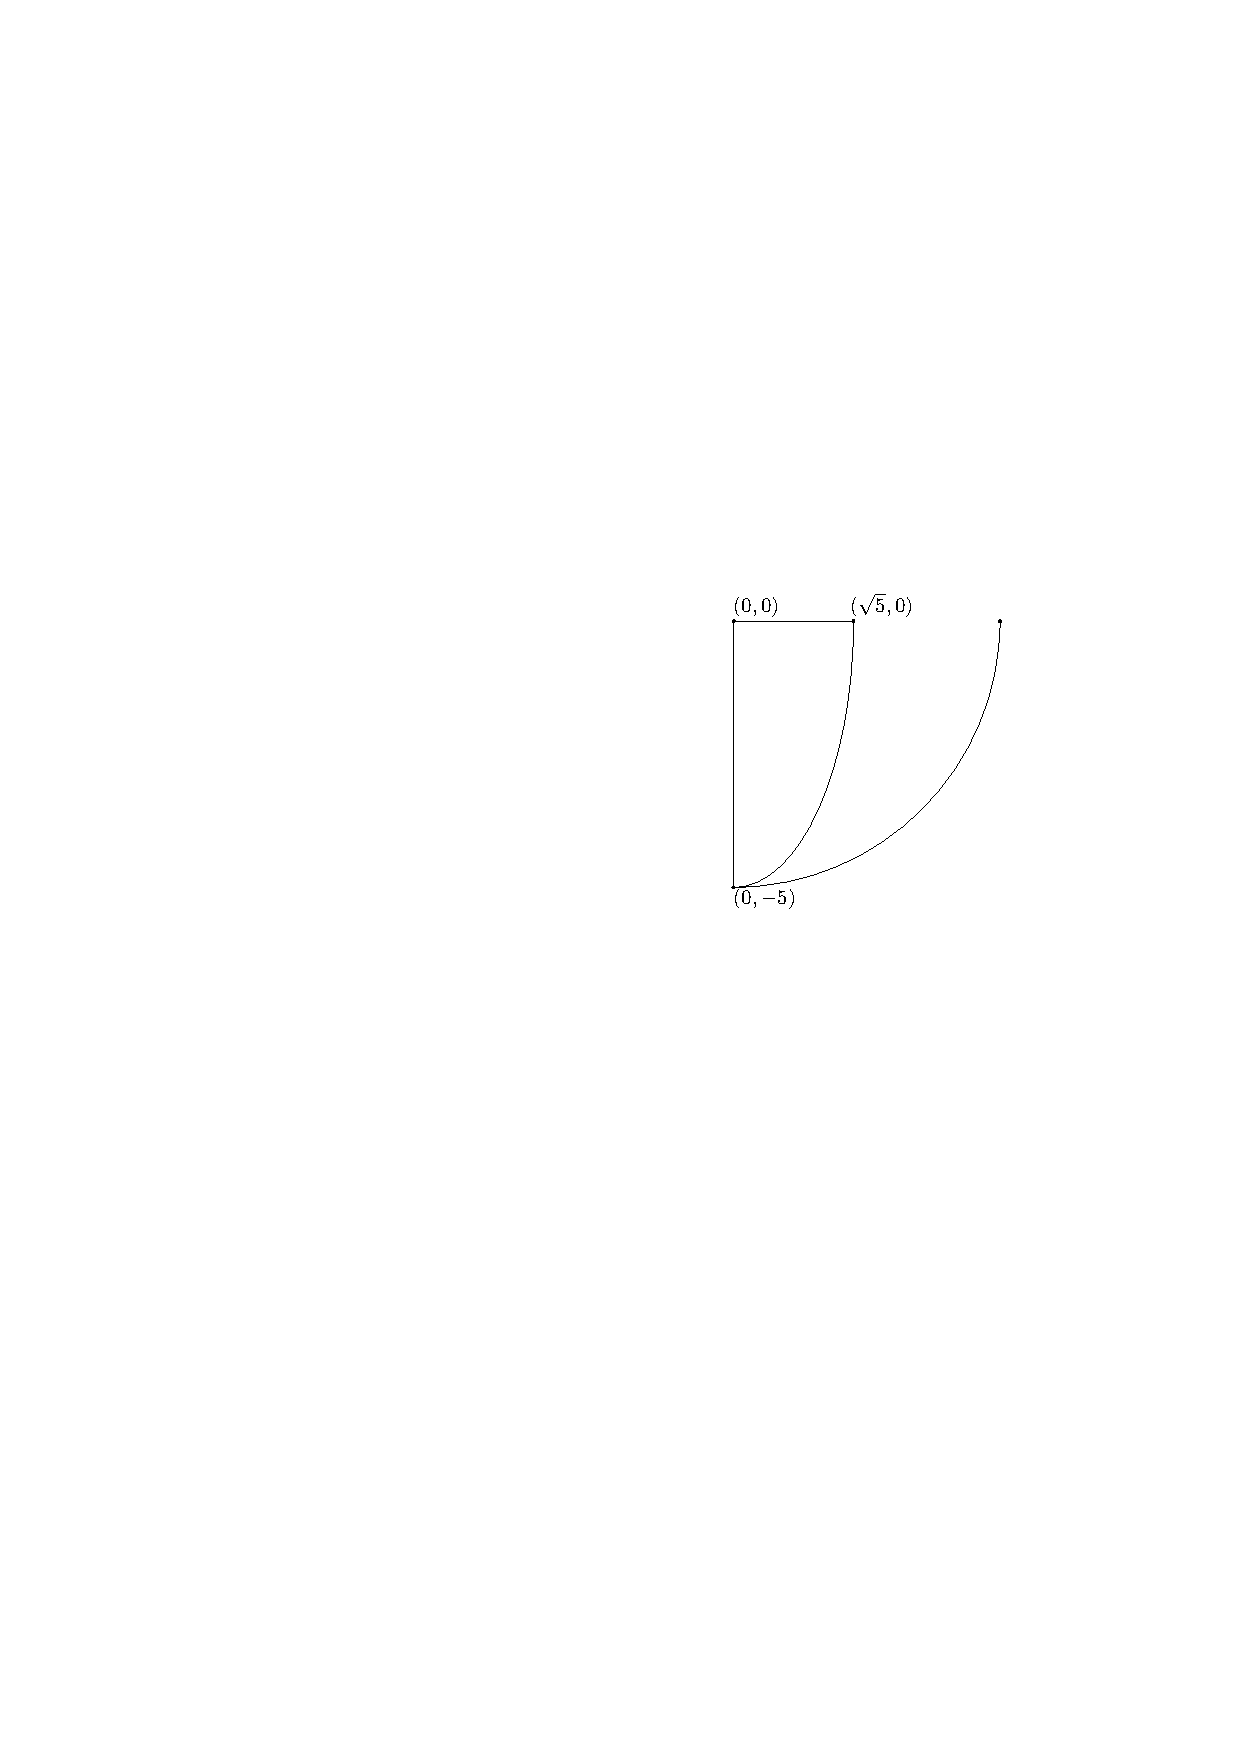
\includegraphics[width=0.7\linewidth,page=1]{includegraphics/ellipse_example_values.pdf}
	\end{subfigure}
	\caption{Illustration of equation \ref{eq:ellipse_example}}\label{im:ellipse5}
\end{figure}
For the orientation of the ellipse arcs, we will pick the values of $x$ and $y$ adequately. The extreme values of equation \ref{eq:ellipse_example} are $(0,-5)$ and $(\sqrt{5},0)$, it would fit right in instead of a circular quarter arc with radius $5$. If $5$ was the longest vertical segment, it would be sufficient to stretch the drawing by $\sqrt{5}$.
This implies - given a height $l$, serving as radius for the original circular arcs - following equation:
\begin{align}
\frac{x^2}{l}+\frac{y^2}{l^2} = 1&&x,-y \in \mathbb{R}_+\label{eq:ellipse_general}
\end{align}
With following extreme values: $(0,-l)$ and $(\sqrt{l},0)$. For every vertical segment of length $l'$, we could compute the ellipse given by equation \ref{eq:ellipse_general} and by gauging our values for $x$ and $y$ we could pick the right orientation of the arc from its appropriate quadrant. 
\subsubsection*{Correctness}
The argument is very similar to the \grqq Boxing\grqq. Instead of a square box, we will deal with rectangles of size $w\times h$. Let $l$ be the longest vertical segment in a given orthogonal drawing $\Gamma_G$. By stretching the drawing by the factor of $\sqrt{|l|}$, every vertical line segment $v$ now has a free rectangle area of size $\sqrt{|l|} \times |v|$ left and right from it. Therefore, $v$ has a free rectangle area of size $\sqrt{|v|} \times |v|$, since $|v| \leq |l| \Rightarrow |\sqrt{v}| \leq |\sqrt{l}|$, guaranteeing the free area for the ellipse arc substitution and a drawing of size $\Rho(n\cdot\sqrt{n})\times\Rho(n)$ in the worst case.
%Utilizing the strict monotonicity of the square root function, we would now be able to stretch the original Kandinsky drawing by the square root of the longest vertical segment $\sqrt{l}$, guaranteeing $\Rho(n\cdot\sqrt{n})\times\Rho(n)$ area.
\subsubsection*{Readability}
Using arcs from ellipses seems to be a good idea at first since we can actually save space, even in the worst case. But using those arcs decrease the readability of a drawing, the bigger the longest vertical segment gets.
\begin{figure}[H]
	\centering
	\begin{subfigure}{0.3\textwidth}
		\centering
		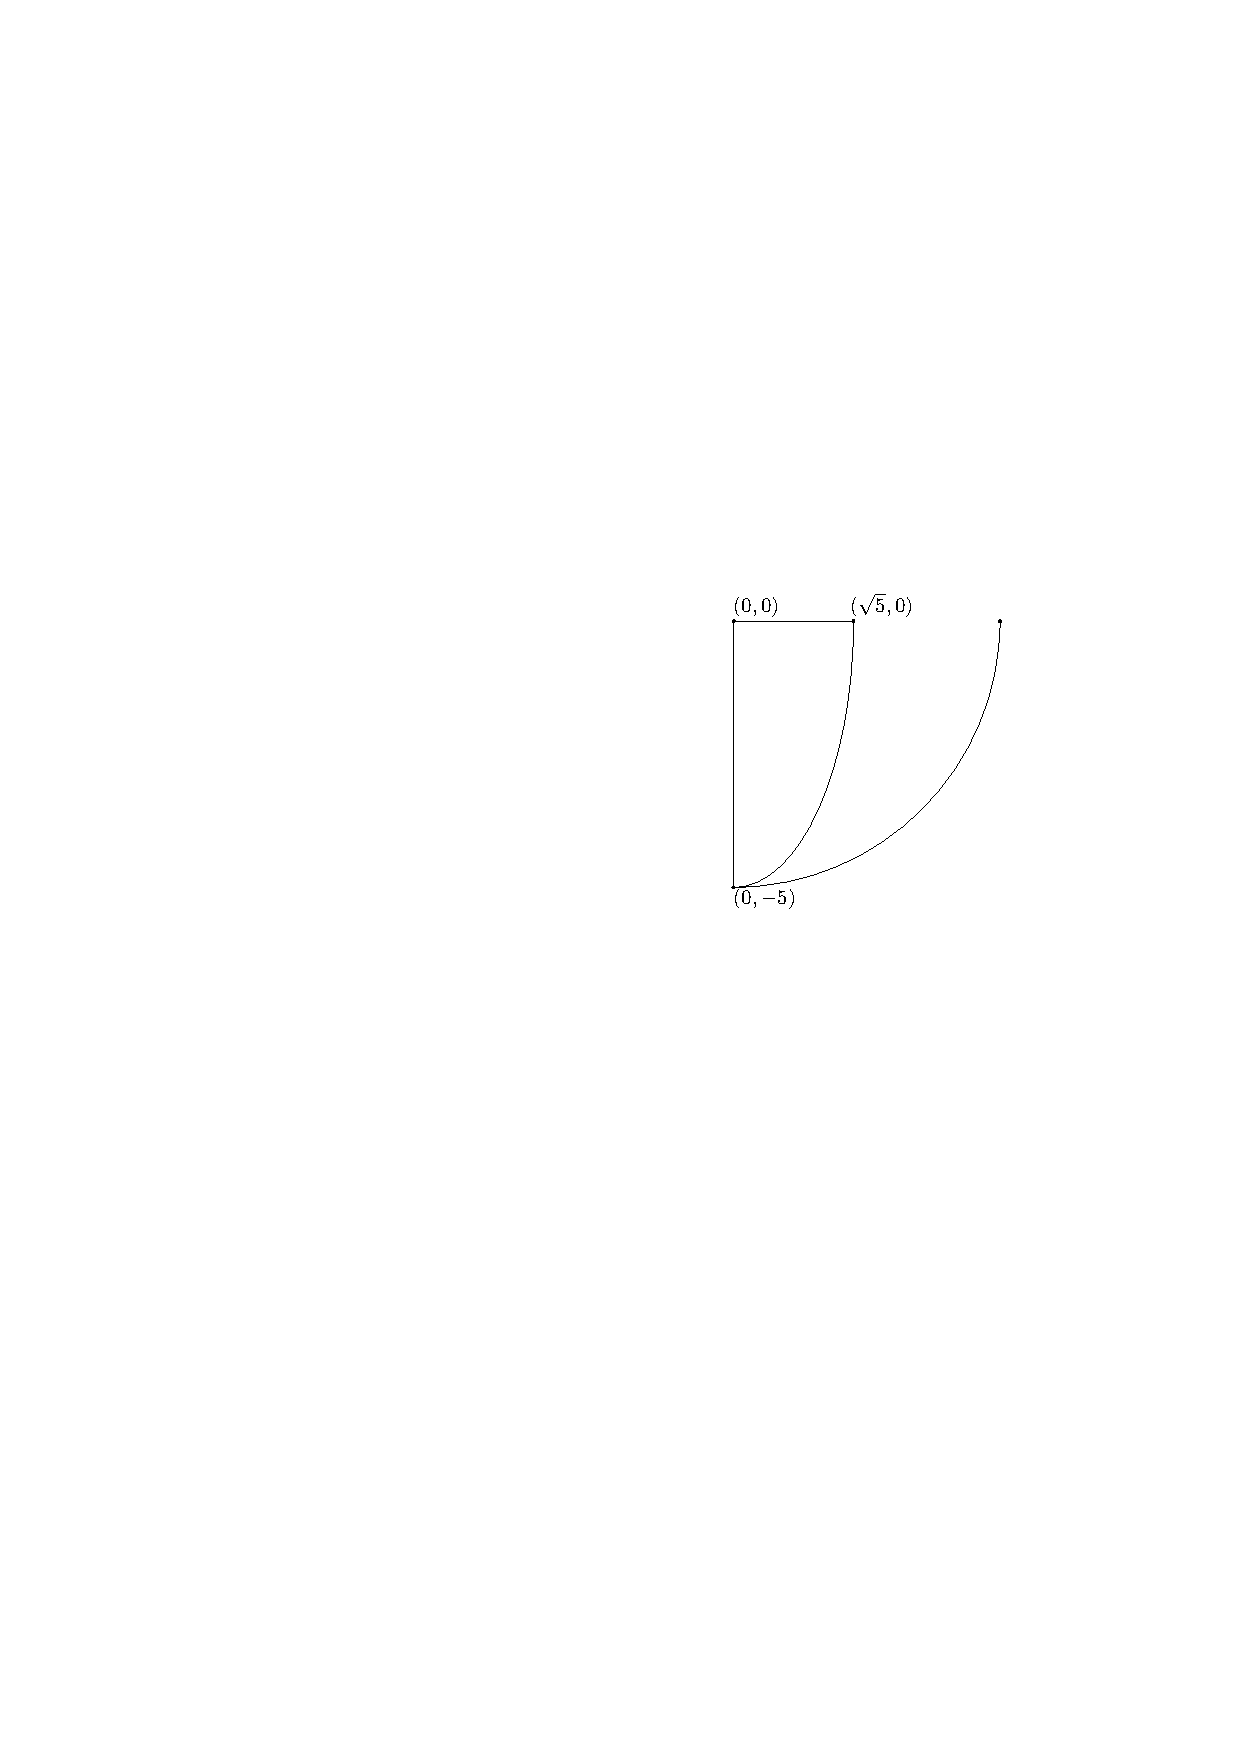
\includegraphics[width=0.7\linewidth,page=1]{includegraphics/ellipse_example_values.pdf}
		\caption{$|l'| = 5$}
	\end{subfigure}
	\begin{subfigure}{0.3\textwidth}
		\centering
		\includegraphics[width=0.7\linewidth,page=2]{includegraphics/ellipse_example_values.pdf}
		\caption{$|l'| = 100$}
	\end{subfigure}
	\begin{subfigure}{0.3\textwidth}
		\centering
		\includegraphics[width=0.7\linewidth,page=3]{includegraphics/ellipse_example_values.pdf}
		\caption{$|l'| = 1000$}
	\end{subfigure}
	\caption{Illustration of increasing values for the vertical segment result in very steep ellipse arcs}
\end{figure}
\subsubsection{Combination of circular arcs and vertical segments}
Maybe a slightly different approach would be to set the width traveled by $\sqrt{l'}$, whereas $l'$ describes the length of the horizontal segment. A combination of a circular arc with radius $\sqrt{l'}$ and a vertical segment of length $l'-\sqrt{l'}$ would illustrate the outgoing edge more precisely. 
\begin{figure}[H]
	\centering
	\begin{subfigure}{0.3\textwidth}
		\centering
		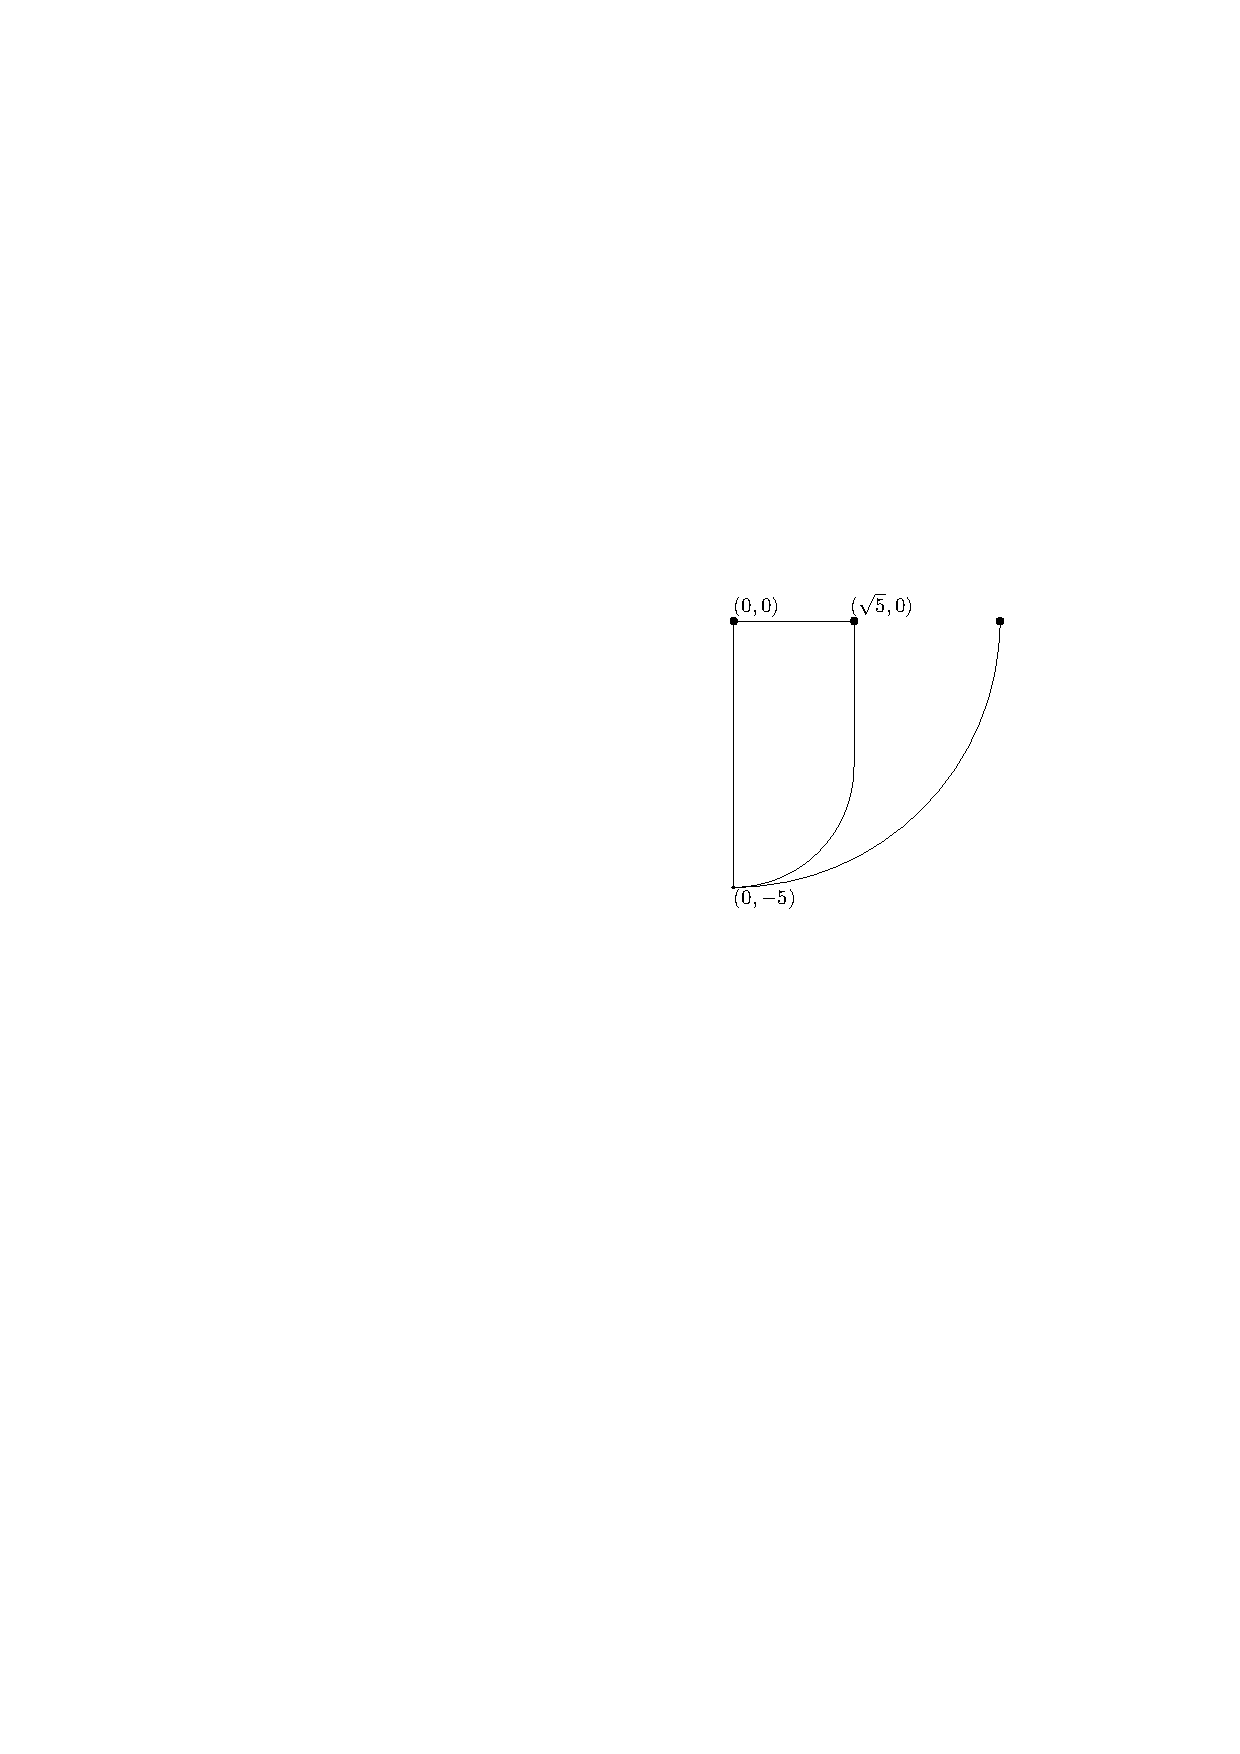
\includegraphics[width=0.7\linewidth,page=1]{includegraphics/vSMOG_example_values.pdf}
		\caption{$|l'| = 5$}
	\end{subfigure}
	\begin{subfigure}{0.3\textwidth}
		\centering
		\includegraphics[width=0.7\linewidth,page=2]{includegraphics/vSMOG_example_values.pdf}
		\caption{$|l'| = 100$}
	\end{subfigure}
	\begin{subfigure}{0.3\textwidth}
		\centering
		\includegraphics[width=0.7\linewidth,page=3]{includegraphics/vSMOG_example_values.pdf}
		\caption{$|l'| = 1000$}
	\end{subfigure}
	\caption{Illustration of increasing values for the vertical segment with the combination of a circular arc and a vertical segment}
\end{figure}
On one hand, we would still take $\Rho(n\cdot\sqrt{n})\times\Rho(n)$ area in the worst case but on the other hand the complexity in this altered smooth orthogonal layout would significantly increase.